\documentclass[twoside,twocolumn,a4paper]{article}

\usepackage[latin1]{inputenc}
\usepackage[T1]{fontenc}
\usepackage{mathptmx}
\usepackage{graphicx}
\usepackage{estylf_en}

% In order to work with mathematical environments (propositions, theorems, etc.), the following packages are suggested:
%\usepackage{amsmath,amsthm}
\usepackage{amsmath, amsthm}
\usepackage{amsfonts}

\hyphenation{pro-per-ties}
\hyphenation{ge-ne-ral-ly}
\hyphenation{pre-fe-ren-ces}
\hyphenation{u-sing}
\hyphenation{pu-nish-ment}

\newcommand{\Pow}{\mathcal{P}}
\newcommand{\N}{\operatorname{N}}
\newcommand{\bool}{\operatorname*{\mathcal{B}}}
\newcommand{\Pos}{\operatorname{Pos}}
\newcommand{\Nec}{\operatorname{Nec}}
\newcommand{\T}{\mathcal{T}}

\begin{document}

\title{Possibilistic evaluation of fuzzy temporal intervals}

%*******************************************************
% REMARKS ABOUT THE AUTHORS
%*******************************************************
% In order to write the name and surname of an author in the the same line, the symbol ~ will be required.
%*******************************************************
% If all the authors share the same affiliation, the following commands are suggested to avoid the superscript:
% \author{Name1~Surname1}
% \address{Address1}{autor1@e-mail1.com}
%*******************************************************

\author[1]{Jos\'e Enrique~Pons}
\author[2]{Antoon~Bronselaer}
\author[1]{Olga~Pons}
\author[2]{Guy~De Tr\'e}
\address[1]{Department of Computer Science and Artificial Intelligence,University of Granada, Spain}{\{jpons,opc\}@decsai.ugr.es}
\address[2]{Department of Telecommunications and Information Processing, Ghent University, Belgium}{\{Antoon.Bronselaer,Guy.De.Tre\}@telin.ugent.be}

\maketitle

\begin{abstract}
Possibility theory tries to quantify the uncertainty caused by incomplete information. A specific case of incomplete information is that of ill-known temporal intervals. The study of these fuzzy intervals is of particular interest in temporal database research. In order to optimize the storage of fuzzy temporal intervals, some transformations have been proposed. In this paper we analyze the possibilistic evaluation of the ill-known temporal intervals and the proposed transformations. It is shown how the reasoning behind the transformations implies a possibilistic information lost. 

\textbf{Keywords:} Possibility theory, ill-known values, ill-known sets, intervals, temporal databases.\vspace{9mm}
\end{abstract}

\section{INTRODUCTION}

The connection of possibility theory \cite{Zadeh78},\cite{Shackle61},\cite{Gaines75} and fuzzy sets has been studied among others by Zadeh \cite{Zadeh65}. This connection establishes two different natures for a fuzzy set \cite{Dubois97}:
\begin{itemize}
\item
\textbf{Conjunctive nature}: The fuzzyfication of a regular set. This interpretation corresponds with the following two semantics: \textit{Degree of preference} and \textit{degree of similarity}.
\item
\textbf{Disjunctive nature}: In this case, the disjunctive nature indicates a description of incomplete knowledge. This interpretation corresponds with the semantics for the \textit{degree of uncertainty}.
\end{itemize}

The disjunctive nature can be seen as an additional connection between fuzzy set theory and possibility theory. Dubois and Prade \cite{Dubois88b} have studied the problem of inferring uncertainty about sets from uncertainty about values. They explain how the incomplete knowledge about a set can be represented as a possibility distribution over a universe $\Pow \left(U \right)$, the power set over the universe $U$. The main drawback of the approach is the large overhead that such a distribution introduces.  A mechanism for the propagation of uncertainty about set elements towards uncertainty about sets is introduced in \textit{'Possibilistic evaluation of sets'} \cite{Pon11}.

There are several proposals in the literature for inferring uncertainty about sets from uncertainty about values. It is of particular interest for fuzzy temporal databases, the application on temporal intervals. The transformation from two ill-known temporal points to a ill-known set has been discussed in \cite{Garrido2009}. In this work we will analyze the major pitfalls of these approaches and the benefit of using the mechanism proposed in \cite{Pon11}.

The paper is organized as follows. In Section \ref{sec:preliminaries}, some preliminaries and concepts about the possibilistic evaluation framework and the temporal databases are presented. The proposal for interval evaluation is done in Section \ref{sec:interval-eval}. In Section \ref{sec:analysis}, the analysis among the different transformations is done. Finally, Section \ref{sec:conclusions} presents the main conclusions and some lines for the future work in this research.


\section{\label{sec:preliminaries}PRELIMINARIES}
In this section we will introduce some basic concepts. First of all, an introduction to possibility theory is explained. Then, the concepts of fuzzy numbers and fuzzy intervals introduced by Dubois and Prade \cite{Dubois1983} are discussed. Finally, a brief introduction to temporal databases is done.

\subsection{\label{subsec:possibilistic-variables}Possibilistic variables}
A possibilistic variable $X$ over a universe $U$ is defined as a variable taking exactly one value in $U$, but for which this value is (partially) unknown. The possibility distribution $\pi_X$ gives the available knowledge about the value that $X$ takes. For each $u\in U$, $\pi_X(u)$ represents the possibility that $X$ takes the value $u$.

It is important to understand the difference between the following two concepts:
\begin{itemize}
\item
A \emph{possibilistic variable} $X$ is bounded to take only one value , but this value is not known due to incomplete knowledge. 
\item
An \emph{ill-known set}~\cite{Dubois88b}: a possibilistic variable defined over the universe $\Pow(U)$.
\end{itemize}

Note that while a possibilistic variable refers to one (partially) unknown value, an ill-known set is a crisp set but, for some reason, (partially) unknown.


\subsection{\label{subsec:fuzzy-numbers}Fuzzy numbers and fuzzy intervals}
Dubois and Prade~\cite{Dubois1983} proposed the following definition of \emph{fuzzy interval}.
%\begin{definition}
A fuzzy interval is a fuzzy set $M$ on the set of real numbers $\mathbb{R}$ such that:
\begin{eqnarray}
\forall (u,v)\in\mathbb{R}^2:&\\
\nonumber
\forall w \in [u,v]:&\mu_M(w) \geq\min(\mu_M(u),\mu_M(v))  \\
\exists m \in \mathbb{R}:& \mu_M(m)=1 
\end{eqnarray}
%\end{definition}
If $m$ is unique, then $M$ is referred to as a \emph{fuzzy number}, instead of a \emph{fuzzy interval}. In other words, if the core of a fuzzy interval is a singleton, it can be seen as a fuzzy number. In their work, Dubois and Prade propose four different functions (two possibility and two necessity functions) to asses the position of a fuzzy number N relative to  a fuzzy number M taken as a reference.

The most convenient representation for the membership function of a fuzzy number is a triangular function. The membership function $\mu_M$ for the fuzzy set $M$ has also the properties of convexity and normalization. Three values represent a triangular function: %(see Figure~\ref{fig:triangular}):
\begin{itemize}
\item
$D$ is the singleton value in the core of $\mu_M(x)$.
\item
$D-a$ is the lower value in the support of $\mu_M(x)$. 
\item
$D+b$ is the upper value in the support of $\mu_M(x)$.
\end{itemize}
Note that the values $a$ and $b$ are values in the underlying ordered domain. E.g. $(a,b) \in \mathbb{R}^2$. The notation for a triangular function adopted here is $[D,a,b]$.
%\begin{figure}[h!]
%  \centering
%  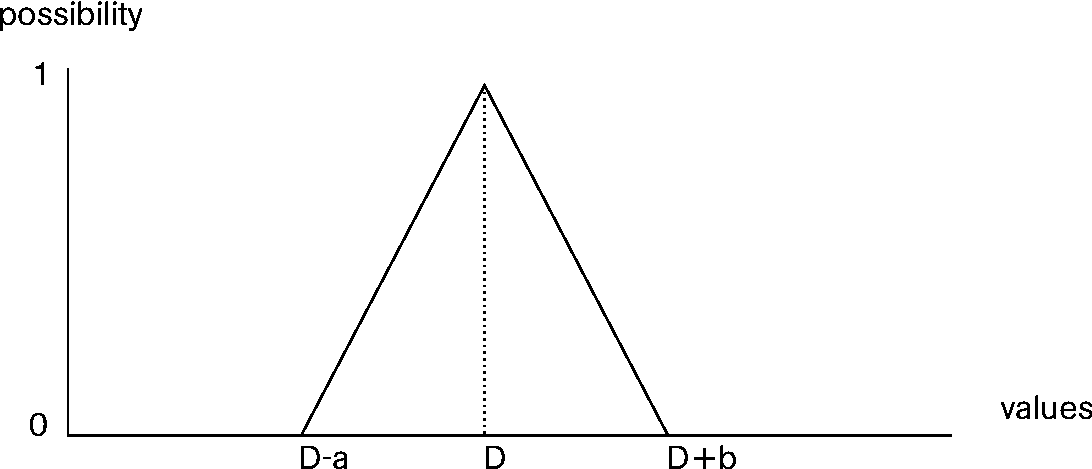
\includegraphics[scale=0.4]{graphs/triangular.pdf}
%  \caption{Triangular function.}
%  \label{fig:triangular}
%\end{figure}

The most simple representation for the membership function of a fuzzy interval is a trapezoidal function. This membership function $\mu_T$ for the fuzzy interval $T$ is convex and normalized. Four values represent a trapezoidal membership function %(figure  \ref{fig:trapezoidal}):
 $\left[\alpha,\ \beta,\ \gamma,\ \delta\right]$. The membership function is given by:

%\begin{align}
%\mu_T(x)
%\begin{cases}
%1 & \mbox{ if } x \in [\beta,\gamma] \\
%0 & \mbox{ if } x > \delta \vee x < \alpha \\
%\frac{x-\alpha}{\beta - \alpha} & \mbox{ if } x \in [\alpha,\beta[ \\
%\frac{\delta -x}{\delta - \gamma} & \mbox{ if } x \in ]\gamma,\delta] \\
%\end{cases}
%\end{align}
%
%\begin{figure}[h!]
%  \centering
%  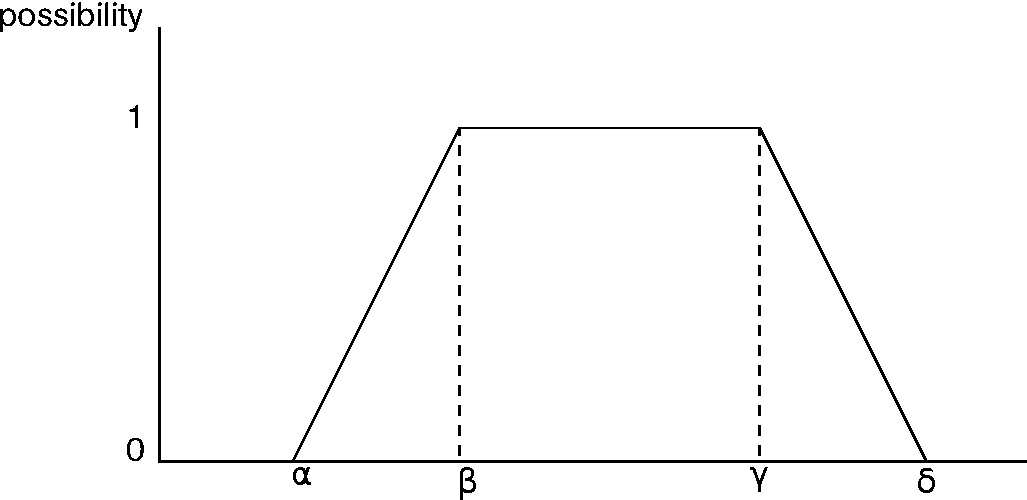
\includegraphics[scale=0.4]{graphs/trapezoidalDistribution.pdf}
%  \caption{Trapezoidal distribution.}
%  \label{fig:trapezoidal}
%\end{figure}



\subsection{\label{subsec:temporal}Temporal databases}
%In this section, the proposed reasoning is applied to the specific context of intervals on the real line. This setting is of specific interest in the context of fuzzy temporal databases.
A temporal database \cite{Dyreson1994} is a database that manages some aspects of time in its schema. A \textbf{chronon} is the shortest duration of time supported by the database. The time can be represented either as points or intervals \cite{655777}. Fuzzy temporal models \cite{4481150} are proposed when the time points or intervals are not precisely known. There are proposals for the  fuzzyfication of the time point \cite{Dubois89} and the fuzzyfication of the time interval \cite{Garrido2009}.\\
Allen \cite{Allen:1983:MKT:182.358434} studied the comparison between two crisp time intervals. For fuzzy intervals, several proposals \cite{4481150}, \cite{springerlink:10.1007/978-3-540-39964-3_57},\cite{10.1109/TIME.2004.1314418} have been done.


%Time granularity is also associated with the representation of the time. A granularity is the result of partitioning on the set of chronons. The conversion among granularities is a common issue within temporal databases \cite{Lin97efficientconversion}. Granularity is the basis of some systems \cite{Cru97},\cite{624013}.


Despite of user-defined time (an uninterpreted attribute; supported in the standard SQL2 \cite{Mel93}), there are 3 types of time in a temporal database:

\begin{itemize}
	\item
	\textbf{Transaction time}: The time when the fact is stored in the database.
	\item
	\textbf{Valid time}: The time when the fact is true in the modelled reality.
	\item
	\textbf{Decision time} \cite{Nascimento95decisiontime}: The time when an event was decided to happen. 
	\end{itemize}
	
	 The  database model can be then classified into: transaction time \cite{Ston87},\cite{Jensen:1991:IIM:627283.627484}, Valid time, bi-temporal \cite{Snodgrass:1984:TQL:588011.588041}(both valid and transaction time) or tri-temporal \cite{Nascimento95decisiontime} (valid, transaction and decision time).

Fuzzy temporal models \cite{4481150} deal with time points \cite{Dubois89} or intervals \cite{Garrido2009} that are ill-known. Some fuzzy temporal models assume that the time stored in the database is an interval. The temporal interval is represented by two ill-known time points: $X$  an ill-known starting point and $Y$ an ill-known ending point. The interval $\left[X,Y\right]$ is not a fuzzy interval but an ill-known interval: it is a crisp interval but it is partially unknown which values are in this interval.




\section{\label{sec:interval-eval}INTERVAL EVALUATION BY ILL-KNOWN CONSTRAINTS}
The problem of the interval evaluation is explained in \cite{Pon11}: For a crisp interval $I = \left[ a, b \right]$, we want to know if all points in this interval reside between the boundaries of the ill-known interval $\left[ X , Y \right]$, where $X,Y$ are ill-known values on the set of real numbers $\mathbb{R}$, and $\lambda$ is the evaluation function. The following expressions compute the possibility and the necessity: 

\begin{eqnarray}
\label{eq:interval-pos}
\Pos\left(\lambda([a,b])\right)=\\
\nonumber
\min\bigg(\sup_{a\geq w}\pi_{X}(w),\sup_{b\leq w}\pi_{Y}(w)\bigg)\\
\label{eq:interval-nec}
\Nec\left(\lambda([a,b])\right)=\\
\nonumber
\min\bigg(\inf_{a<w}1-\pi_{X}(w),\inf_{b>w}1-\pi_{Y}(w)\bigg).
\end{eqnarray}

Note that the expressions in \eqref{eq:interval-pos},\eqref{eq:interval-nec} cannot be simplified in a more efficient expressions. %repensar
An ill-known point is given by a triangular membership function. The ill-known values $X$ and $Y$ are represented by the triangular membership functions $\left[D_X,a_X,b_X \right]$ and $\left[D_Y,a_Y,b_Y \right]$ respectively. The equation \eqref{eq:interval-pos} is derived to:

\begin{eqnarray}
\label{eq:interval-pos-triangular-a}
\sup_{a\geq w}\pi_{X}(w)=
\begin{cases}
0 & \mbox{\ if\ } a \leq \left( D_X - a_X \right) \\
1 & \mbox{\ if\ } a \geq D_X \\
 \frac{a-D_X+a_X}{a_X} & \mbox{\ if\ } a \in \left(D_X-a_X,D_X \right)
\end{cases}\\
\label{eq:interval-pos-triangular-b}
\sup_{b\leq w}\pi_{Y}(w)=
\begin{cases}
0 & \mbox{\ if\ } b \geq \left( D_Y + b_Y \right) \\
1 & \mbox{\ if\ } b \leq D_Y \\
 \frac{D_X+b_X-b}{b_X} & \mbox{\ if\ } b \in \left(D_Y,D_Y+b_Y \right) 
\end{cases}
\end{eqnarray}

The necessity expression of \eqref{eq:interval-nec} for triangular membership functions is given by:

\begin{eqnarray}
\label{eq:interval-nec-triangular-a}
\inf_{a<w}1-\pi_{X}(w)=
\begin{cases}
0 & \mbox{\ if\ } a \leq  D_X   \\
1 & \mbox{\ if\ } a \geq \left( D_X+b_X \right) \\
\frac{a}{b_X}- \frac{D_X}{b_X} & \mbox{\ if\ } a \in \left(D_X,D_X+b_X \right)
\end{cases}\\
\label{eq:interval-nec-triangular-b}
\inf_{b>w}1-\pi_{Y}(w)=
\begin{cases}
0 & \mbox{\ if\ } b \geq  D_Y \\
1 & \mbox{\ if\ } b \leq \left( D_Y - a_Y \right) \\
 \frac{D_Y-b}{a_X} & \mbox{\ if\ } b \in \left(D_Y,D_Y+b_Y \right) 
\end{cases}
\end{eqnarray}

\paragraph{Example} Consider the ill-known values $X = \left[3, 2, 1\right]$ and $Y = \left[7, 2, 3 \right]$. The knowledge about the evaluation of the interval $\left[a, b \right]$ w.r.t. $X$ and $Y$ is given by the expressions \eqref{eq:interval-pos},\eqref{eq:interval-nec}.  Figure \ref{fig:interval-rep} shows the graphical representation for the ill-known values $X$ and $Y$. The representation for equations \eqref{eq:interval-pos-triangular-a},\eqref{eq:interval-pos-triangular-b},\eqref{eq:interval-nec-triangular-a},\eqref{eq:interval-nec-triangular-b} are shown respectively in figures \ref{fig:interval_membership_pos_a},\ref{fig:interval_membership_pos_b},\ref{fig:interval_membership_nec_a},\ref{fig:interval_membership_nec_b}.

Consider now that the value for the interval $\left[a, b \right]$ is $\left[2, 6 \right]$. The evaluation for the possibility and necessity are:

\begin{eqnarray}
\label{eq:interval-pos}
\nonumber
\Pos\left(\lambda([3,6])\right)=\min(1,1)= 1\\
\label{eq:interval-nec}
\nonumber
\Nec\left(\lambda([3,6])\right)=\min(1,0.5 ) = 0.5
\end{eqnarray}

The main difference between this proposal and the transformations is that this framework always allows to obtain both possibility and necessity measures for each temporal comparison. In this case, there are the following possibilities:

\begin{itemize}
\item
$\Pos(\lambda([a,b])) = 0 \rightarrow \Nec(\lambda([a,b])) = 0$: The interval $[a,b]$ is not contained the fuzzy interval $[X,Y]$.
\item
$\Pos(\lambda([a,b])) > 0 $, $\Nec(\lambda([a,b])) = 0$: The interval $[a,b]$ is contained the fuzzy interval $[X,Y]$ but it is not inside the cores of both $X$ and $Y$.
\item
$\Pos(\lambda([a,b])) = 1 $, $\Nec(\lambda([a,b])) = 1$: The interval $[a,b]$ is contained the fuzzy interval $[X,Y]$ and it is inside the cores of both $X$ and $Y$.
\end{itemize}

\begin{figure}[h!]
\centering
%%Created by jPicEdt 1.4.1_03: mixed JPIC-XML/LaTeX format
%%Wed Nov 23 16:38:02 CET 2011
%%Begin JPIC-XML
%<?xml version="1.0" standalone="yes"?>
%<jpic x-min="-2.5" x-max="60" y-min="-2.5" y-max="32.5" auto-bounding="true">
%<multicurve fill-style= "none"
%	 points= "(0,0);(0,0);(55,0);(55,0)"
%	 right-arrow= "head"
%	 />
%<multicurve fill-style= "none"
%	 points= "(0,0);(0,0);(0,30);(0,30)"
%	 right-arrow= "head"
%	 />
%<text fill-style= "none"
%	 text-vert-align= "center-v"
%	 anchor-point= "(-2.5,27.5)"
%	 text-frame= "noframe"
%	 text-hor-align= "center-h"
%	 right-arrow= "head"
%	 >
%1
%</text>
%<text fill-style= "none"
%	 text-vert-align= "center-v"
%	 anchor-point= "(-2.5,0)"
%	 text-frame= "noframe"
%	 text-hor-align= "center-h"
%	 right-arrow= "head"
%	 >
%0
%</text>
%<text fill-style= "none"
%	 text-vert-align= "center-v"
%	 anchor-point= "(15,32.5)"
%	 text-rotation= "135"
%	 text-frame= "noframe"
%	 text-hor-align= "center-h"
%	 right-arrow= "head"
%	 >
%Membership Degree
%</text>
%<text fill-style= "none"
%	 text-vert-align= "center-v"
%	 anchor-point= "(10,-2.5)"
%	 text-frame= "noframe"
%	 text-hor-align= "center-h"
%	 right-arrow= "head"
%	 >
%2
%</text>
%<text fill-style= "none"
%	 text-vert-align= "center-v"
%	 anchor-point= "(15,-2.5)"
%	 text-frame= "noframe"
%	 text-hor-align= "center-h"
%	 right-arrow= "head"
%	 >
%3
%</text>
%<text fill-style= "none"
%	 text-vert-align= "center-v"
%	 anchor-point= "(20,-2.5)"
%	 text-frame= "noframe"
%	 text-hor-align= "center-h"
%	 right-arrow= "head"
%	 >
%4
%</text>
%<text fill-style= "none"
%	 text-vert-align= "center-v"
%	 anchor-point= "(25,-2.5)"
%	 text-frame= "noframe"
%	 text-hor-align= "center-h"
%	 right-arrow= "head"
%	 >
%5
%</text>
%<text fill-style= "none"
%	 text-vert-align= "center-v"
%	 anchor-point= "(30,-2.5)"
%	 text-frame= "noframe"
%	 text-hor-align= "center-h"
%	 right-arrow= "head"
%	 >
%6
%</text>
%<text fill-style= "none"
%	 text-vert-align= "center-v"
%	 anchor-point= "(35,-2.5)"
%	 text-frame= "noframe"
%	 text-hor-align= "center-h"
%	 right-arrow= "head"
%	 >
%7
%</text>
%<text fill-style= "none"
%	 text-vert-align= "center-v"
%	 anchor-point= "(40,-2.5)"
%	 text-frame= "noframe"
%	 text-hor-align= "center-h"
%	 right-arrow= "head"
%	 >
%8
%</text>
%<text fill-style= "none"
%	 text-vert-align= "center-v"
%	 anchor-point= "(45,-2.5)"
%	 text-frame= "noframe"
%	 text-hor-align= "center-h"
%	 right-arrow= "head"
%	 >
%9
%</text>
%<text fill-style= "none"
%	 text-vert-align= "center-v"
%	 anchor-point= "(50,-2.5)"
%	 text-frame= "noframe"
%	 text-hor-align= "center-h"
%	 right-arrow= "head"
%	 >
%10
%</text>
%<text fill-style= "none"
%	 text-vert-align= "center-v"
%	 anchor-point= "(5,-2.5)"
%	 text-frame= "noframe"
%	 text-hor-align= "center-h"
%	 right-arrow= "head"
%	 >
%1
%</text>
%<multicurve fill-style= "none"
%	 points= "(5,0);(5,0);(15,27.5);(15,27.5)"
%	 />
%<multicurve fill-style= "none"
%	 points= "(15,27.5);(15,27.5);(20,0);(20,0)"
%	 />
%<multicurve fill-style= "none"
%	 points= "(25,0);(25,0);(35,27.5);(35,27.5)"
%	 />
%<multicurve fill-style= "none"
%	 points= "(35,27.5);(35,27.5);(50,0);(50,0)"
%	 />
%<text fill-style= "none"
%	 text-vert-align= "center-v"
%	 anchor-point= "(10,25)"
%	 text-frame= "noframe"
%	 text-hor-align= "center-h"
%	 >
%X
%</text>
%<text fill-style= "none"
%	 text-vert-align= "center-v"
%	 anchor-point= "(40,25)"
%	 text-frame= "noframe"
%	 text-hor-align= "center-h"
%	 >
%Y
%</text>
%<text fill-style= "none"
%	 text-vert-align= "center-v"
%	 anchor-point= "(60,0)"
%	 text-frame= "noframe"
%	 text-hor-align= "center-h"
%	 >
%Time
%</text>
%</jpic>
%%End JPIC-XML
%LaTeX-picture environment using emulated lines and arcs
%You can rescale the whole picture (to 80% for instance) by using the command \def\JPicScale{0.8}
\ifx\JPicScale\undefined\def\JPicScale{1}\fi
\unitlength \JPicScale mm
\begin{picture}(60,32.5)(0,0)
\linethickness{0.3mm}
\put(0,0){\line(1,0){55}}
\put(55,0){\vector(1,0){0.12}}
\linethickness{0.3mm}
\put(0,0){\line(0,1){30}}
\put(0,30){\vector(0,1){0.12}}
\put(-2.5,27.5){\makebox(0,0)[cc]{1}}

\put(-2.5,0){\makebox(0,0)[cc]{0}}

\put(15,32.5){\makebox(0,0)[cc]{Membership Degree}}

\put(10,-2.5){\makebox(0,0)[cc]{2}}

\put(15,-2.5){\makebox(0,0)[cc]{3}}

\put(20,-2.5){\makebox(0,0)[cc]{4}}

\put(25,-2.5){\makebox(0,0)[cc]{5}}

\put(30,-2.5){\makebox(0,0)[cc]{6}}

\put(35,-2.5){\makebox(0,0)[cc]{7}}

\put(40,-2.5){\makebox(0,0)[cc]{8}}

\put(45,-2.5){\makebox(0,0)[cc]{9}}

\put(50,-2.5){\makebox(0,0)[cc]{10}}

\put(5,-2.5){\makebox(0,0)[cc]{1}}

\linethickness{0.3mm}
\multiput(5,0)(0.12,0.33){83}{\line(0,1){0.33}}
\linethickness{0.3mm}
\multiput(15,27.5)(0.12,-0.65){42}{\line(0,-1){0.65}}
\linethickness{0.3mm}
\multiput(25,0)(0.12,0.33){83}{\line(0,1){0.33}}
\linethickness{0.3mm}
\multiput(35,27.5)(0.12,-0.22){125}{\line(0,-1){0.22}}
\put(10,25){\makebox(0,0)[cc]{X}}

\put(40,25){\makebox(0,0)[cc]{Y}}

\put(60,0){\makebox(0,0)[cc]{Time}}

\end{picture}

\caption{Triangular membership functions for the two ill-known time points $X$ and $Y$.}
\label{fig:interval-rep}
\end{figure}

\begin{figure}[h!]
\centering
%%Created by jPicEdt 1.4.1_03: mixed JPIC-XML/LaTeX format
%%Thu Nov 24 10:44:33 CET 2011
%%Begin JPIC-XML
%<?xml version="1.0" standalone="yes"?>
%<jpic x-min="-2.5" x-max="60" y-min="-2.5" y-max="32.5" auto-bounding="true">
%<multicurve right-arrow= "head"
%	 fill-style= "none"
%	 points= "(0,0);(0,0);(55,0);(55,0)"
%	 />
%<multicurve right-arrow= "head"
%	 fill-style= "none"
%	 points= "(0,0);(0,0);(0,30);(0,30)"
%	 />
%<text right-arrow= "head"
%	 fill-style= "none"
%	 text-vert-align= "center-v"
%	 anchor-point= "(-2.5,27.5)"
%	 text-frame= "noframe"
%	 text-hor-align= "center-h"
%	 >
%1
%</text>
%<text right-arrow= "head"
%	 fill-style= "none"
%	 text-vert-align= "center-v"
%	 anchor-point= "(-2.5,0)"
%	 text-frame= "noframe"
%	 text-hor-align= "center-h"
%	 >
%0
%</text>
%<text right-arrow= "head"
%	 fill-style= "none"
%	 text-vert-align= "center-v"
%	 anchor-point= "(15,32.5)"
%	 text-rotation= "135"
%	 text-frame= "noframe"
%	 text-hor-align= "center-h"
%	 >
%Membership Degree
%</text>
%<text right-arrow= "head"
%	 fill-style= "none"
%	 text-vert-align= "center-v"
%	 anchor-point= "(10,-2.5)"
%	 text-frame= "noframe"
%	 text-hor-align= "center-h"
%	 >
%2
%</text>
%<text right-arrow= "head"
%	 fill-style= "none"
%	 text-vert-align= "center-v"
%	 anchor-point= "(15,-2.5)"
%	 text-frame= "noframe"
%	 text-hor-align= "center-h"
%	 >
%3
%</text>
%<text right-arrow= "head"
%	 fill-style= "none"
%	 text-vert-align= "center-v"
%	 anchor-point= "(20,-2.5)"
%	 text-frame= "noframe"
%	 text-hor-align= "center-h"
%	 >
%4
%</text>
%<text right-arrow= "head"
%	 fill-style= "none"
%	 text-vert-align= "center-v"
%	 anchor-point= "(25,-2.5)"
%	 text-frame= "noframe"
%	 text-hor-align= "center-h"
%	 >
%5
%</text>
%<text right-arrow= "head"
%	 fill-style= "none"
%	 text-vert-align= "center-v"
%	 anchor-point= "(30,-2.5)"
%	 text-frame= "noframe"
%	 text-hor-align= "center-h"
%	 >
%6
%</text>
%<text right-arrow= "head"
%	 fill-style= "none"
%	 text-vert-align= "center-v"
%	 anchor-point= "(35,-2.5)"
%	 text-frame= "noframe"
%	 text-hor-align= "center-h"
%	 >
%7
%</text>
%<text right-arrow= "head"
%	 fill-style= "none"
%	 text-vert-align= "center-v"
%	 anchor-point= "(40,-2.5)"
%	 text-frame= "noframe"
%	 text-hor-align= "center-h"
%	 >
%8
%</text>
%<text right-arrow= "head"
%	 fill-style= "none"
%	 text-vert-align= "center-v"
%	 anchor-point= "(45,-2.5)"
%	 text-frame= "noframe"
%	 text-hor-align= "center-h"
%	 >
%9
%</text>
%<text right-arrow= "head"
%	 fill-style= "none"
%	 text-vert-align= "center-v"
%	 anchor-point= "(50,-2.5)"
%	 text-frame= "noframe"
%	 text-hor-align= "center-h"
%	 >
%10
%</text>
%<text right-arrow= "head"
%	 fill-style= "none"
%	 text-vert-align= "center-v"
%	 anchor-point= "(5,-2.5)"
%	 text-frame= "noframe"
%	 text-hor-align= "center-h"
%	 >
%1
%</text>
%<multicurve fill-style= "none"
%	 stroke-dasharray= "1;1"
%	 points= "(5,0);(5,0);(15,27.5);(15,27.5)"
%	 stroke-style= "dashed"
%	 />
%<multicurve fill-style= "none"
%	 stroke-dasharray= "1;1"
%	 points= "(15,27.5);(15,27.5);(52.5,27.5);(52.5,27.5)"
%	 stroke-style= "dashed"
%	 />
%<text fill-style= "none"
%	 text-vert-align= "center-v"
%	 anchor-point= "(60,0)"
%	 text-frame= "noframe"
%	 text-hor-align= "center-h"
%	 >
%Time
%</text>
%<text fill-style= "none"
%	 text-vert-align= "center-v"
%	 anchor-point= "(37.5,22.5)"
%	 text-frame= "noframe"
%	 text-hor-align= "center-h"
%	 >
%$\sup_{a\geq w}\pi_{X}(w)$
%</text>
%</jpic>
%%End JPIC-XML
%LaTeX-picture environment using emulated lines and arcs
%You can rescale the whole picture (to 80% for instance) by using the command \def\JPicScale{0.8}
\ifx\JPicScale\undefined\def\JPicScale{1}\fi
\unitlength \JPicScale mm
\begin{picture}(60,32.5)(0,0)
\linethickness{0.3mm}
\put(0,0){\line(1,0){55}}
\put(55,0){\vector(1,0){0.12}}
\linethickness{0.3mm}
\put(0,0){\line(0,1){30}}
\put(0,30){\vector(0,1){0.12}}
\put(-2.5,27.5){\makebox(0,0)[cc]{1}}

\put(-2.5,0){\makebox(0,0)[cc]{0}}

\put(15,32.5){\makebox(0,0)[cc]{Membership Degree}}

\put(10,-2.5){\makebox(0,0)[cc]{2}}

\put(15,-2.5){\makebox(0,0)[cc]{3}}

\put(20,-2.5){\makebox(0,0)[cc]{4}}

\put(25,-2.5){\makebox(0,0)[cc]{5}}

\put(30,-2.5){\makebox(0,0)[cc]{6}}

\put(35,-2.5){\makebox(0,0)[cc]{7}}

\put(40,-2.5){\makebox(0,0)[cc]{8}}

\put(45,-2.5){\makebox(0,0)[cc]{9}}

\put(50,-2.5){\makebox(0,0)[cc]{10}}

\put(5,-2.5){\makebox(0,0)[cc]{1}}

\linethickness{0.3mm}
\multiput(5,0)(0.69,1.9){15}{\multiput(0,0)(0.11,0.32){3}{\line(0,1){0.32}}}
\linethickness{0.3mm}
\multiput(15,27.5)(2.03,0){19}{\line(1,0){1.01}}
\put(60,0){\makebox(0,0)[cc]{Time}}

\put(37.5,22.5){\makebox(0,0)[cc]{$\sup_{a\geq w}\pi_{X}(w)$}}

\end{picture}

\caption{Membership function for $\sup_{a\geq w}\pi_{X}(w)$.}
\label{fig:interval_membership_pos_a}
\end{figure}

\begin{figure}[h!]
\centering
%%Created by jPicEdt 1.4.1_03: mixed JPIC-XML/LaTeX format
%%Thu Nov 24 10:55:36 CET 2011
%%Begin JPIC-XML
%<?xml version="1.0" standalone="yes"?>
%<jpic x-min="-2.5" x-max="60" y-min="-2.5" y-max="32.5" auto-bounding="true">
%<multicurve right-arrow= "head"
%	 fill-style= "none"
%	 points= "(0,0);(0,0);(55,0);(55,0)"
%	 />
%<multicurve right-arrow= "head"
%	 fill-style= "none"
%	 points= "(0,0);(0,0);(0,30);(0,30)"
%	 />
%<text right-arrow= "head"
%	 fill-style= "none"
%	 text-vert-align= "center-v"
%	 anchor-point= "(-2.5,27.5)"
%	 text-frame= "noframe"
%	 text-hor-align= "center-h"
%	 >
%1
%</text>
%<text right-arrow= "head"
%	 fill-style= "none"
%	 text-vert-align= "center-v"
%	 anchor-point= "(-2.5,0)"
%	 text-frame= "noframe"
%	 text-hor-align= "center-h"
%	 >
%0
%</text>
%<text right-arrow= "head"
%	 fill-style= "none"
%	 text-vert-align= "center-v"
%	 anchor-point= "(15,32.5)"
%	 text-rotation= "135"
%	 text-frame= "noframe"
%	 text-hor-align= "center-h"
%	 >
%Membership Degree
%</text>
%<text right-arrow= "head"
%	 fill-style= "none"
%	 text-vert-align= "center-v"
%	 anchor-point= "(10,-2.5)"
%	 text-frame= "noframe"
%	 text-hor-align= "center-h"
%	 >
%2
%</text>
%<text right-arrow= "head"
%	 fill-style= "none"
%	 text-vert-align= "center-v"
%	 anchor-point= "(15,-2.5)"
%	 text-frame= "noframe"
%	 text-hor-align= "center-h"
%	 >
%3
%</text>
%<text right-arrow= "head"
%	 fill-style= "none"
%	 text-vert-align= "center-v"
%	 anchor-point= "(20,-2.5)"
%	 text-frame= "noframe"
%	 text-hor-align= "center-h"
%	 >
%4
%</text>
%<text right-arrow= "head"
%	 fill-style= "none"
%	 text-vert-align= "center-v"
%	 anchor-point= "(25,-2.5)"
%	 text-frame= "noframe"
%	 text-hor-align= "center-h"
%	 >
%5
%</text>
%<text right-arrow= "head"
%	 fill-style= "none"
%	 text-vert-align= "center-v"
%	 anchor-point= "(30,-2.5)"
%	 text-frame= "noframe"
%	 text-hor-align= "center-h"
%	 >
%6
%</text>
%<text right-arrow= "head"
%	 fill-style= "none"
%	 text-vert-align= "center-v"
%	 anchor-point= "(35,-2.5)"
%	 text-frame= "noframe"
%	 text-hor-align= "center-h"
%	 >
%7
%</text>
%<text right-arrow= "head"
%	 fill-style= "none"
%	 text-vert-align= "center-v"
%	 anchor-point= "(40,-2.5)"
%	 text-frame= "noframe"
%	 text-hor-align= "center-h"
%	 >
%8
%</text>
%<text right-arrow= "head"
%	 fill-style= "none"
%	 text-vert-align= "center-v"
%	 anchor-point= "(45,-2.5)"
%	 text-frame= "noframe"
%	 text-hor-align= "center-h"
%	 >
%9
%</text>
%<text right-arrow= "head"
%	 fill-style= "none"
%	 text-vert-align= "center-v"
%	 anchor-point= "(50,-2.5)"
%	 text-frame= "noframe"
%	 text-hor-align= "center-h"
%	 >
%10
%</text>
%<text right-arrow= "head"
%	 fill-style= "none"
%	 text-vert-align= "center-v"
%	 anchor-point= "(5,-2.5)"
%	 text-frame= "noframe"
%	 text-hor-align= "center-h"
%	 >
%1
%</text>
%<multicurve fill-style= "none"
%	 stroke-dasharray= "1;1"
%	 points= "(0,27.5);(0,27.5);(35,27.5);(35,27.5)"
%	 stroke-style= "dashed"
%	 />
%<multicurve fill-style= "none"
%	 stroke-dasharray= "1;1"
%	 points= "(35,27.5);(35,27.5);(50,0);(50,0)"
%	 stroke-style= "dashed"
%	 />
%<text fill-style= "none"
%	 text-vert-align= "center-v"
%	 anchor-point= "(60,0)"
%	 text-frame= "noframe"
%	 text-hor-align= "center-h"
%	 >
%Time
%</text>
%<text fill-style= "none"
%	 text-vert-align= "center-v"
%	 anchor-point= "(27.5,22.5)"
%	 text-frame= "noframe"
%	 text-hor-align= "center-h"
%	 >
%$\sup_{b\leq w}\pi_{Y}(w)$
%</text>
%</jpic>
%%End JPIC-XML
%LaTeX-picture environment using emulated lines and arcs
%You can rescale the whole picture (to 80% for instance) by using the command \def\JPicScale{0.8}
\ifx\JPicScale\undefined\def\JPicScale{1}\fi
\unitlength \JPicScale mm
\begin{picture}(60,32.5)(0,0)
\linethickness{0.3mm}
\put(0,0){\line(1,0){55}}
\put(55,0){\vector(1,0){0.12}}
\linethickness{0.3mm}
\put(0,0){\line(0,1){30}}
\put(0,30){\vector(0,1){0.12}}
\put(-2.5,27.5){\makebox(0,0)[cc]{1}}

\put(-2.5,0){\makebox(0,0)[cc]{0}}

\put(15,32.5){\makebox(0,0)[cc]{Membership Degree}}

\put(10,-2.5){\makebox(0,0)[cc]{2}}

\put(15,-2.5){\makebox(0,0)[cc]{3}}

\put(20,-2.5){\makebox(0,0)[cc]{4}}

\put(25,-2.5){\makebox(0,0)[cc]{5}}

\put(30,-2.5){\makebox(0,0)[cc]{6}}

\put(35,-2.5){\makebox(0,0)[cc]{7}}

\put(40,-2.5){\makebox(0,0)[cc]{8}}

\put(45,-2.5){\makebox(0,0)[cc]{9}}

\put(50,-2.5){\makebox(0,0)[cc]{10}}

\put(5,-2.5){\makebox(0,0)[cc]{1}}

\linethickness{0.3mm}
\multiput(0,27.5)(2,0){18}{\line(1,0){1}}
\linethickness{0.3mm}
\multiput(35,27.5)(0.97,-1.77){16}{\multiput(0,0)(0.12,-0.22){4}{\line(0,-1){0.22}}}
\put(60,0){\makebox(0,0)[cc]{Time}}

\put(27.5,22.5){\makebox(0,0)[cc]{$\sup_{b\leq w}\pi_{Y}(w)$}}

\end{picture}

\caption{Membership function for $\sup_{b\leq w}\pi_{Y}(w)$.}
\label{fig:interval_membership_pos_b}
\end{figure}

\begin{figure}[h!]
\centering
%%Created by jPicEdt 1.4.1_03: mixed JPIC-XML/LaTeX format
%%Thu Nov 24 10:59:01 CET 2011
%%Begin JPIC-XML
%<?xml version="1.0" standalone="yes"?>
%<jpic x-min="-2.5" x-max="60" y-min="-2.5" y-max="32.5" auto-bounding="true">
%<multicurve right-arrow= "head"
%	 fill-style= "none"
%	 points= "(0,0);(0,0);(55,0);(55,0)"
%	 />
%<multicurve right-arrow= "head"
%	 fill-style= "none"
%	 points= "(0,0);(0,0);(0,30);(0,30)"
%	 />
%<text right-arrow= "head"
%	 fill-style= "none"
%	 text-vert-align= "center-v"
%	 anchor-point= "(-2.5,27.5)"
%	 text-frame= "noframe"
%	 text-hor-align= "center-h"
%	 >
%1
%</text>
%<text right-arrow= "head"
%	 fill-style= "none"
%	 text-vert-align= "center-v"
%	 anchor-point= "(-2.5,0)"
%	 text-frame= "noframe"
%	 text-hor-align= "center-h"
%	 >
%0
%</text>
%<text right-arrow= "head"
%	 fill-style= "none"
%	 text-vert-align= "center-v"
%	 anchor-point= "(15,32.5)"
%	 text-rotation= "135"
%	 text-frame= "noframe"
%	 text-hor-align= "center-h"
%	 >
%Membership Degree
%</text>
%<text right-arrow= "head"
%	 fill-style= "none"
%	 text-vert-align= "center-v"
%	 anchor-point= "(10,-2.5)"
%	 text-frame= "noframe"
%	 text-hor-align= "center-h"
%	 >
%2
%</text>
%<text right-arrow= "head"
%	 fill-style= "none"
%	 text-vert-align= "center-v"
%	 anchor-point= "(15,-2.5)"
%	 text-frame= "noframe"
%	 text-hor-align= "center-h"
%	 >
%3
%</text>
%<text right-arrow= "head"
%	 fill-style= "none"
%	 text-vert-align= "center-v"
%	 anchor-point= "(20,-2.5)"
%	 text-frame= "noframe"
%	 text-hor-align= "center-h"
%	 >
%4
%</text>
%<text right-arrow= "head"
%	 fill-style= "none"
%	 text-vert-align= "center-v"
%	 anchor-point= "(25,-2.5)"
%	 text-frame= "noframe"
%	 text-hor-align= "center-h"
%	 >
%5
%</text>
%<text right-arrow= "head"
%	 fill-style= "none"
%	 text-vert-align= "center-v"
%	 anchor-point= "(30,-2.5)"
%	 text-frame= "noframe"
%	 text-hor-align= "center-h"
%	 >
%6
%</text>
%<text right-arrow= "head"
%	 fill-style= "none"
%	 text-vert-align= "center-v"
%	 anchor-point= "(35,-2.5)"
%	 text-frame= "noframe"
%	 text-hor-align= "center-h"
%	 >
%7
%</text>
%<text right-arrow= "head"
%	 fill-style= "none"
%	 text-vert-align= "center-v"
%	 anchor-point= "(40,-2.5)"
%	 text-frame= "noframe"
%	 text-hor-align= "center-h"
%	 >
%8
%</text>
%<text right-arrow= "head"
%	 fill-style= "none"
%	 text-vert-align= "center-v"
%	 anchor-point= "(45,-2.5)"
%	 text-frame= "noframe"
%	 text-hor-align= "center-h"
%	 >
%9
%</text>
%<text right-arrow= "head"
%	 fill-style= "none"
%	 text-vert-align= "center-v"
%	 anchor-point= "(50,-2.5)"
%	 text-frame= "noframe"
%	 text-hor-align= "center-h"
%	 >
%10
%</text>
%<text right-arrow= "head"
%	 fill-style= "none"
%	 text-vert-align= "center-v"
%	 anchor-point= "(5,-2.5)"
%	 text-frame= "noframe"
%	 text-hor-align= "center-h"
%	 >
%1
%</text>
%<multicurve fill-style= "none"
%	 points= "(5,0);(5,0);(15,27.5);(15,27.5)"
%	 />
%<multicurve fill-style= "none"
%	 points= "(15,27.5);(15,27.5);(20,0);(20,0)"
%	 />
%<text fill-style= "none"
%	 text-vert-align= "center-v"
%	 anchor-point= "(10,25)"
%	 text-frame= "noframe"
%	 text-hor-align= "center-h"
%	 >
%X
%</text>
%<text fill-style= "none"
%	 text-vert-align= "center-v"
%	 anchor-point= "(60,0)"
%	 text-frame= "noframe"
%	 text-hor-align= "center-h"
%	 >
%Time
%</text>
%<multicurve fill-style= "none"
%	 stroke-dasharray= "1;1"
%	 points= "(15,0);(15,0);(20,27.5);(20,27.5)"
%	 stroke-style= "dashed"
%	 />
%<multicurve fill-style= "none"
%	 stroke-dasharray= "1;1"
%	 points= "(20,27.5);(20,27.5);(50,27.5);(50,27.5)"
%	 stroke-style= "dashed"
%	 />
%<text fill-style= "none"
%	 text-vert-align= "center-v"
%	 anchor-point= "(42.5,25)"
%	 text-frame= "noframe"
%	 text-hor-align= "center-h"
%	 >
%$\inf_{a&lt;w}1-\pi_{X}(w)$
%</text>
%</jpic>
%%End JPIC-XML
%LaTeX-picture environment using emulated lines and arcs
%You can rescale the whole picture (to 80% for instance) by using the command \def\JPicScale{0.8}
\ifx\JPicScale\undefined\def\JPicScale{1}\fi
\unitlength \JPicScale mm
\begin{picture}(60,32.5)(0,0)
\linethickness{0.3mm}
\put(0,0){\line(1,0){55}}
\put(55,0){\vector(1,0){0.12}}
\linethickness{0.3mm}
\put(0,0){\line(0,1){30}}
\put(0,30){\vector(0,1){0.12}}
\put(-2.5,27.5){\makebox(0,0)[cc]{1}}

\put(-2.5,0){\makebox(0,0)[cc]{0}}

\put(15,32.5){\makebox(0,0)[cc]{Membership Degree}}

\put(10,-2.5){\makebox(0,0)[cc]{2}}

\put(15,-2.5){\makebox(0,0)[cc]{3}}

\put(20,-2.5){\makebox(0,0)[cc]{4}}

\put(25,-2.5){\makebox(0,0)[cc]{5}}

\put(30,-2.5){\makebox(0,0)[cc]{6}}

\put(35,-2.5){\makebox(0,0)[cc]{7}}

\put(40,-2.5){\makebox(0,0)[cc]{8}}

\put(45,-2.5){\makebox(0,0)[cc]{9}}

\put(50,-2.5){\makebox(0,0)[cc]{10}}

\put(5,-2.5){\makebox(0,0)[cc]{1}}

\linethickness{0.3mm}
\multiput(5,0)(0.12,0.33){83}{\line(0,1){0.33}}
\linethickness{0.3mm}
\multiput(15,27.5)(0.12,-0.65){42}{\line(0,-1){0.65}}
\put(10,25){\makebox(0,0)[cc]{X}}

\put(60,0){\makebox(0,0)[cc]{Time}}

\linethickness{0.3mm}
\multiput(15,0)(0.37,2.04){14}{\multiput(0,0)(0.09,0.51){2}{\line(0,1){0.51}}}
\linethickness{0.3mm}
\multiput(20,27.5)(1.94,0){16}{\line(1,0){0.97}}
\put(42.5,25){\makebox(0,0)[cc]{$\inf_{a<w}1-\pi_{X}(w)$}}

\end{picture}

\caption{Membership function for $\inf_{a<w}1-\pi_{X}(w)$.}
\label{fig:interval_membership_nec_a}
\end{figure}

\begin{figure}[h!]
\centering
%%Created by jPicEdt 1.4.1_03: mixed JPIC-XML/LaTeX format
%%Thu Nov 24 11:00:59 CET 2011
%%Begin JPIC-XML
%<?xml version="1.0" standalone="yes"?>
%<jpic x-min="-2.5" x-max="60" y-min="-2.5" y-max="32.5" auto-bounding="true">
%<multicurve right-arrow= "head"
%	 fill-style= "none"
%	 points= "(0,0);(0,0);(55,0);(55,0)"
%	 />
%<multicurve right-arrow= "head"
%	 fill-style= "none"
%	 points= "(0,0);(0,0);(0,30);(0,30)"
%	 />
%<text right-arrow= "head"
%	 fill-style= "none"
%	 text-vert-align= "center-v"
%	 anchor-point= "(-2.5,27.5)"
%	 text-frame= "noframe"
%	 text-hor-align= "center-h"
%	 >
%1
%</text>
%<text right-arrow= "head"
%	 fill-style= "none"
%	 text-vert-align= "center-v"
%	 anchor-point= "(-2.5,0)"
%	 text-frame= "noframe"
%	 text-hor-align= "center-h"
%	 >
%0
%</text>
%<text right-arrow= "head"
%	 fill-style= "none"
%	 text-vert-align= "center-v"
%	 anchor-point= "(15,32.5)"
%	 text-rotation= "135"
%	 text-frame= "noframe"
%	 text-hor-align= "center-h"
%	 >
%Membership Degree
%</text>
%<text right-arrow= "head"
%	 fill-style= "none"
%	 text-vert-align= "center-v"
%	 anchor-point= "(10,-2.5)"
%	 text-frame= "noframe"
%	 text-hor-align= "center-h"
%	 >
%2
%</text>
%<text right-arrow= "head"
%	 fill-style= "none"
%	 text-vert-align= "center-v"
%	 anchor-point= "(15,-2.5)"
%	 text-frame= "noframe"
%	 text-hor-align= "center-h"
%	 >
%3
%</text>
%<text right-arrow= "head"
%	 fill-style= "none"
%	 text-vert-align= "center-v"
%	 anchor-point= "(20,-2.5)"
%	 text-frame= "noframe"
%	 text-hor-align= "center-h"
%	 >
%4
%</text>
%<text right-arrow= "head"
%	 fill-style= "none"
%	 text-vert-align= "center-v"
%	 anchor-point= "(25,-2.5)"
%	 text-frame= "noframe"
%	 text-hor-align= "center-h"
%	 >
%5
%</text>
%<text right-arrow= "head"
%	 fill-style= "none"
%	 text-vert-align= "center-v"
%	 anchor-point= "(30,-2.5)"
%	 text-frame= "noframe"
%	 text-hor-align= "center-h"
%	 >
%6
%</text>
%<text right-arrow= "head"
%	 fill-style= "none"
%	 text-vert-align= "center-v"
%	 anchor-point= "(35,-2.5)"
%	 text-frame= "noframe"
%	 text-hor-align= "center-h"
%	 >
%7
%</text>
%<text right-arrow= "head"
%	 fill-style= "none"
%	 text-vert-align= "center-v"
%	 anchor-point= "(40,-2.5)"
%	 text-frame= "noframe"
%	 text-hor-align= "center-h"
%	 >
%8
%</text>
%<text right-arrow= "head"
%	 fill-style= "none"
%	 text-vert-align= "center-v"
%	 anchor-point= "(45,-2.5)"
%	 text-frame= "noframe"
%	 text-hor-align= "center-h"
%	 >
%9
%</text>
%<text right-arrow= "head"
%	 fill-style= "none"
%	 text-vert-align= "center-v"
%	 anchor-point= "(50,-2.5)"
%	 text-frame= "noframe"
%	 text-hor-align= "center-h"
%	 >
%10
%</text>
%<text right-arrow= "head"
%	 fill-style= "none"
%	 text-vert-align= "center-v"
%	 anchor-point= "(5,-2.5)"
%	 text-frame= "noframe"
%	 text-hor-align= "center-h"
%	 >
%1
%</text>
%<multicurve fill-style= "none"
%	 points= "(25,0);(25,0);(35,27.5);(35,27.5)"
%	 />
%<multicurve fill-style= "none"
%	 points= "(35,27.5);(35,27.5);(50,0);(50,0)"
%	 />
%<text fill-style= "none"
%	 text-vert-align= "center-v"
%	 anchor-point= "(40,25)"
%	 text-frame= "noframe"
%	 text-hor-align= "center-h"
%	 >
%Y
%</text>
%<text fill-style= "none"
%	 text-vert-align= "center-v"
%	 anchor-point= "(60,0)"
%	 text-frame= "noframe"
%	 text-hor-align= "center-h"
%	 >
%Time
%</text>
%<multicurve fill-style= "none"
%	 stroke-dasharray= "1;1"
%	 points= "(35,0);(35,0);(25,27.5);(25,27.5)"
%	 stroke-style= "dashed"
%	 />
%<multicurve fill-style= "none"
%	 stroke-dasharray= "1;1"
%	 points= "(25,27.5);(25,27.5);(0,27.5);(0,27.5)"
%	 stroke-style= "dashed"
%	 />
%<text fill-style= "none"
%	 text-vert-align= "center-v"
%	 stroke-dasharray= "1;1"
%	 anchor-point= "(22.5,25)"
%	 stroke-style= "dashed"
%	 text-frame= "noframe"
%	 text-hor-align= "center-h"
%	 >
%$inf_{b&gt;w}1-\pi_{Y}(w)$
%</text>
%</jpic>
%%End JPIC-XML
%LaTeX-picture environment using emulated lines and arcs
%You can rescale the whole picture (to 80% for instance) by using the command \def\JPicScale{0.8}
\ifx\JPicScale\undefined\def\JPicScale{1}\fi
\unitlength \JPicScale mm
\begin{picture}(60,32.5)(0,0)
\linethickness{0.3mm}
\put(0,0){\line(1,0){55}}
\put(55,0){\vector(1,0){0.12}}
\linethickness{0.3mm}
\put(0,0){\line(0,1){30}}
\put(0,30){\vector(0,1){0.12}}
\put(-2.5,27.5){\makebox(0,0)[cc]{1}}

\put(-2.5,0){\makebox(0,0)[cc]{0}}

\put(15,32.5){\makebox(0,0)[cc]{Membership Degree}}

\put(10,-2.5){\makebox(0,0)[cc]{2}}

\put(15,-2.5){\makebox(0,0)[cc]{3}}

\put(20,-2.5){\makebox(0,0)[cc]{4}}

\put(25,-2.5){\makebox(0,0)[cc]{5}}

\put(30,-2.5){\makebox(0,0)[cc]{6}}

\put(35,-2.5){\makebox(0,0)[cc]{7}}

\put(40,-2.5){\makebox(0,0)[cc]{8}}

\put(45,-2.5){\makebox(0,0)[cc]{9}}

\put(50,-2.5){\makebox(0,0)[cc]{10}}

\put(5,-2.5){\makebox(0,0)[cc]{1}}

\linethickness{0.3mm}
\multiput(25,0)(0.12,0.33){83}{\line(0,1){0.33}}
\linethickness{0.3mm}
\multiput(35,27.5)(0.12,-0.22){125}{\line(0,-1){0.22}}
\put(40,25){\makebox(0,0)[cc]{Y}}

\put(60,0){\makebox(0,0)[cc]{Time}}

\linethickness{0.3mm}
\multiput(25,27.5)(0.69,-1.9){15}{\multiput(0,0)(0.11,-0.32){3}{\line(0,-1){0.32}}}
\linethickness{0.3mm}
\multiput(0,27.5)(2,0){13}{\line(1,0){1}}
\put(22.5,25){\makebox(0,0)[cc]{$inf_{b>w}1-\pi_{Y}(w)$}}

\end{picture}

\caption{Membership function for $\inf_{b>w}1-\pi_{Y}(w)$.}
\label{fig:interval_membership_nec_b}
\end{figure}

\section{\label{sec:analysis}ANALYSIS OF PROPOSED TRANSFORMATIONS}

There are several proposals to transform two fuzzy numbers that represent an ill-known interval into one fuzzy interval. This reasoning is however not consistent with possibility theory. We provide several arguments to prove this, which have been previously reasoned by Dubois and Prade \cite{Dubois88b}:

\begin{enumerate}
\item
The fuzzy set given by the two fuzzy numbers is conceptually different from a fuzzy set represented by the fuzzy interval. The fuzzy set given by the two fuzzy numbers belong to $\Pow(\mathbb{R})$ while the fuzzy interval obtained after the transformation is not a possibility distribution on $\Pow(\mathbb{R})$  but on $\mathbb{R}$.
\item
In some cases, (like in the convex hull transformation) because of the underlying ordered domain, the membership function provided for the fuzzy interval preserves the possibility. However, the necessity is not preserved at all.
\end{enumerate}

In the next subsections we will analyze the two major approaches: The transformation that preserves the imprecision and the convex hull. 




\subsection{\label{subsubsec:transf-pres-imp}Transformation that preserves the imprecision}
\begin{figure}[h!]
  \centering
  %%Created by jPicEdt 1.4.1_03: mixed JPIC-XML/LaTeX format
%%Mon Nov 28 12:02:12 CET 2011
%%Begin JPIC-XML
%<?xml version="1.0" standalone="yes"?>
%<jpic x-min="-2.5" x-max="60" y-min="-2.5" y-max="75" auto-bounding="true">
%<multicurve fill-style= "none"
%	 points= "(0,40);(0,40);(55,40);(55,40)"
%	 right-arrow= "head"
%	 />
%<multicurve fill-style= "none"
%	 points= "(0,40);(0,40);(0,70);(0,70)"
%	 right-arrow= "head"
%	 />
%<text text-vert-align= "center-v"
%	 anchor-point= "(-2.5,67.5)"
%	 fill-style= "none"
%	 text-frame= "noframe"
%	 text-hor-align= "center-h"
%	 right-arrow= "head"
%	 >
%1
%</text>
%<text text-vert-align= "center-v"
%	 anchor-point= "(-2.5,40)"
%	 fill-style= "none"
%	 text-frame= "noframe"
%	 text-hor-align= "center-h"
%	 right-arrow= "head"
%	 >
%0
%</text>
%<text text-vert-align= "center-v"
%	 anchor-point= "(15,72.5)"
%	 fill-style= "none"
%	 text-rotation= "135"
%	 text-frame= "noframe"
%	 text-hor-align= "center-h"
%	 right-arrow= "head"
%	 >
%Membership Degree
%</text>
%<multicurve fill-style= "none"
%	 points= "(5,40);(5,40);(15,67.5);(15,67.5)"
%	 />
%<multicurve fill-style= "none"
%	 points= "(15,67.5);(15,67.5);(20,40);(20,40)"
%	 />
%<multicurve fill-style= "none"
%	 points= "(25,40);(25,40);(35,67.5);(35,67.5)"
%	 />
%<multicurve fill-style= "none"
%	 points= "(35,67.5);(35,67.5);(50,40);(50,40)"
%	 />
%<text text-vert-align= "center-v"
%	 anchor-point= "(10,65)"
%	 fill-style= "none"
%	 text-frame= "noframe"
%	 text-hor-align= "center-h"
%	 >
%S
%</text>
%<text text-vert-align= "center-v"
%	 anchor-point= "(40,65)"
%	 fill-style= "none"
%	 text-frame= "noframe"
%	 text-hor-align= "center-h"
%	 >
%E
%</text>
%<text text-vert-align= "center-v"
%	 anchor-point= "(60,40)"
%	 fill-style= "none"
%	 text-frame= "noframe"
%	 text-hor-align= "center-h"
%	 >
%Time
%</text>
%<multicurve fill-style= "none"
%	 points= "(0,0);(0,0);(55,0);(55,0)"
%	 right-arrow= "head"
%	 />
%<multicurve fill-style= "none"
%	 points= "(0,0);(0,0);(0,30);(0,30)"
%	 right-arrow= "head"
%	 />
%<text text-vert-align= "center-v"
%	 anchor-point= "(-2.5,27.5)"
%	 fill-style= "none"
%	 text-frame= "noframe"
%	 text-hor-align= "center-h"
%	 right-arrow= "head"
%	 >
%1
%</text>
%<text text-vert-align= "center-v"
%	 anchor-point= "(-2.5,0)"
%	 fill-style= "none"
%	 text-frame= "noframe"
%	 text-hor-align= "center-h"
%	 right-arrow= "head"
%	 >
%0
%</text>
%<text text-vert-align= "center-v"
%	 anchor-point= "(15,32.5)"
%	 fill-style= "none"
%	 text-rotation= "135"
%	 text-frame= "noframe"
%	 text-hor-align= "center-h"
%	 right-arrow= "head"
%	 >
%Membership Degree
%</text>
%<multicurve fill-style= "none"
%	 points= "(5,0);(5,0);(20,27.5);(20,27.5)"
%	 />
%<multicurve fill-style= "none"
%	 points= "(20,27.5);(20,27.5);(25,27.5);(25,27.5)"
%	 />
%<multicurve fill-style= "none"
%	 points= "(25,27.5);(25,27.5);(50,0);(50,0)"
%	 />
%<text text-vert-align= "center-v"
%	 anchor-point= "(60,0)"
%	 fill-style= "none"
%	 text-frame= "noframe"
%	 text-hor-align= "center-h"
%	 >
%Time
%</text>
%<text text-vert-align= "center-v"
%	 stroke-dasharray= "1;1"
%	 anchor-point= "(30,25)"
%	 stroke-style= "dashed"
%	 fill-style= "none"
%	 text-frame= "noframe"
%	 text-hor-align= "center-h"
%	 >
%T
%</text>
%<text text-vert-align= "center-v"
%	 stroke-dasharray= "1;1"
%	 anchor-point= "(12.5,37.5)"
%	 stroke-style= "dashed"
%	 fill-style= "none"
%	 text-frame= "noframe"
%	 text-hor-align= "center-h"
%	 >
%$D_S$
%</text>
%<text text-vert-align= "center-v"
%	 stroke-dasharray= "1;1"
%	 anchor-point= "(5,37.5)"
%	 stroke-style= "dashed"
%	 fill-style= "none"
%	 text-frame= "noframe"
%	 text-hor-align= "center-h"
%	 >
%\tiny{$D_S-a_S$}
%</text>
%<text text-vert-align= "center-v"
%	 stroke-dasharray= "1;1"
%	 anchor-point= "(17.5,-2.5)"
%	 stroke-style= "dashed"
%	 fill-style= "none"
%	 text-frame= "noframe"
%	 text-hor-align= "center-h"
%	 >
%$D_S+b_S$
%</text>
%<text text-vert-align= "center-v"
%	 stroke-dasharray= "1;1"
%	 anchor-point= "(7.5,37.5)"
%	 stroke-style= "dashed"
%	 fill-style= "none"
%	 text-frame= "noframe"
%	 text-hor-align= "center-h"
%	 >
%
%</text>
%<text text-vert-align= "center-v"
%	 stroke-dasharray= "1;1"
%	 anchor-point= "(5,-2.5)"
%	 stroke-style= "dashed"
%	 fill-style= "none"
%	 text-frame= "noframe"
%	 text-hor-align= "center-h"
%	 >
%$D_S-a_S$
%</text>
%<text text-vert-align= "center-v"
%	 stroke-dasharray= "1;1"
%	 anchor-point= "(20,37.5)"
%	 stroke-style= "dashed"
%	 fill-style= "none"
%	 text-frame= "noframe"
%	 text-hor-align= "center-h"
%	 >
%\tiny{$D_S+b_S$}
%</text>
%<text text-vert-align= "center-v"
%	 stroke-dasharray= "1;1"
%	 anchor-point= "(30,-2.5)"
%	 stroke-style= "dashed"
%	 fill-style= "none"
%	 text-frame= "noframe"
%	 text-hor-align= "center-h"
%	 >
%$D_E-a_E$
%</text>
%<text text-vert-align= "center-v"
%	 stroke-dasharray= "1;1"
%	 anchor-point= "(50,-2.5)"
%	 stroke-style= "dashed"
%	 fill-style= "none"
%	 text-frame= "noframe"
%	 text-hor-align= "center-h"
%	 >
%$D_E+b_E$
%</text>
%<text text-vert-align= "center-v"
%	 stroke-dasharray= "1;1"
%	 anchor-point= "(50,-2.5)"
%	 stroke-style= "dashed"
%	 fill-style= "none"
%	 text-frame= "noframe"
%	 text-hor-align= "center-h"
%	 >
%
%</text>
%<text text-vert-align= "center-v"
%	 stroke-dasharray= "1;1"
%	 anchor-point= "(50,-2.5)"
%	 stroke-style= "dashed"
%	 fill-style= "none"
%	 text-frame= "noframe"
%	 text-hor-align= "center-h"
%	 >
%
%</text>
%<multicurve stroke-dasharray= "1;1"
%	 stroke-style= "dashed"
%	 fill-style= "none"
%	 points= "(20,27.5);(20,27.5);(20,0);(20,0)"
%	 />
%<multicurve stroke-dasharray= "1;1"
%	 stroke-style= "dashed"
%	 fill-style= "none"
%	 points= "(25,27.5);(25,27.5);(25,0);(25,0)"
%	 />
%<text text-vert-align= "center-v"
%	 anchor-point= "(37.5,37.5)"
%	 fill-style= "none"
%	 text-frame= "noframe"
%	 text-hor-align= "center-h"
%	 >
%$D_E$
%</text>
%<text text-vert-align= "center-v"
%	 anchor-point= "(27.5,37.5)"
%	 fill-style= "none"
%	 text-frame= "noframe"
%	 text-hor-align= "center-h"
%	 >
%\tiny{$D_E-a_E$}
%</text>
%<text text-vert-align= "center-v"
%	 anchor-point= "(50,37.5)"
%	 fill-style= "none"
%	 text-frame= "noframe"
%	 text-hor-align= "center-h"
%	 >
%\tiny{$D_E+b_E$}
%</text>
%<text text-vert-align= "center-v"
%	 anchor-point= "(52.5,75)"
%	 fill-style= "none"
%	 text-frame= "noframe"
%	 text-hor-align= "center-h"
%	 >
%
%</text>
%</jpic>
%%End JPIC-XML
%LaTeX-picture environment using emulated lines and arcs
%You can rescale the whole picture (to 80% for instance) by using the command \def\JPicScale{0.8}
\ifx\JPicScale\undefined\def\JPicScale{1}\fi
\unitlength \JPicScale mm
\begin{picture}(60,75)(0,0)
\linethickness{0.3mm}
\put(0,40){\line(1,0){55}}
\put(55,40){\vector(1,0){0.12}}
\linethickness{0.3mm}
\put(0,40){\line(0,1){30}}
\put(0,70){\vector(0,1){0.12}}
\put(-2.5,67.5){\makebox(0,0)[cc]{1}}

\put(-2.5,40){\makebox(0,0)[cc]{0}}

\put(15,72.5){\makebox(0,0)[cc]{Membership Degree}}

\linethickness{0.3mm}
\multiput(5,40)(0.12,0.33){83}{\line(0,1){0.33}}
\linethickness{0.3mm}
\multiput(15,67.5)(0.12,-0.65){42}{\line(0,-1){0.65}}
\linethickness{0.3mm}
\multiput(25,40)(0.12,0.33){83}{\line(0,1){0.33}}
\linethickness{0.3mm}
\multiput(35,67.5)(0.12,-0.22){125}{\line(0,-1){0.22}}
\put(10,65){\makebox(0,0)[cc]{S}}

\put(40,65){\makebox(0,0)[cc]{E}}

\put(60,40){\makebox(0,0)[cc]{Time}}

\linethickness{0.3mm}
\put(0,0){\line(1,0){55}}
\put(55,0){\vector(1,0){0.12}}
\linethickness{0.3mm}
\put(0,0){\line(0,1){30}}
\put(0,30){\vector(0,1){0.12}}
\put(-2.5,27.5){\makebox(0,0)[cc]{1}}

\put(-2.5,0){\makebox(0,0)[cc]{0}}

\put(15,32.5){\makebox(0,0)[cc]{Membership Degree}}

\linethickness{0.3mm}
\multiput(5,0)(0.12,0.22){125}{\line(0,1){0.22}}
\linethickness{0.3mm}
\put(20,27.5){\line(1,0){5}}
\linethickness{0.3mm}
\multiput(25,27.5)(0.12,-0.13){208}{\line(0,-1){0.13}}
\put(60,0){\makebox(0,0)[cc]{Time}}

\put(30,25){\makebox(0,0)[cc]{T}}

\put(12.5,37.5){\makebox(0,0)[cc]{$D_S$}}

\put(5,37.5){\makebox(0,0)[cc]{\tiny{$D_S-a_S$}}}

\put(17.5,-2.5){\makebox(0,0)[cc]{$D_S+b_S$}}

\put(7.5,37.5){\makebox(0,0)[cc]{}}

\put(5,-2.5){\makebox(0,0)[cc]{$D_S-a_S$}}

\put(20,37.5){\makebox(0,0)[cc]{\tiny{$D_S+b_S$}}}

\put(30,-2.5){\makebox(0,0)[cc]{$D_E-a_E$}}

\put(50,-2.5){\makebox(0,0)[cc]{$D_E+b_E$}}

\put(50,-2.5){\makebox(0,0)[cc]{}}

\put(50,-2.5){\makebox(0,0)[cc]{}}

\linethickness{0.3mm}
\multiput(20,0)(0,2.04){14}{\line(0,1){1.02}}
\linethickness{0.3mm}
\multiput(25,0)(0,2.04){14}{\line(0,1){1.02}}
\put(37.5,37.5){\makebox(0,0)[cc]{$D_E$}}

\put(27.5,37.5){\makebox(0,0)[cc]{\tiny{$D_E-a_E$}}}

\put(50,37.5){\makebox(0,0)[cc]{\tiny{$D_E+b_E$}}}

\put(52.5,75){\makebox(0,0)[cc]{}}

\end{picture}

  \caption{Transformation of two fuzzy numbers $X$ and $Y$ into one fuzzy interval $T$ preserving the amount of imprecision.}
  \label{fig:transf-pres-imp}
\end{figure}
This transformation has been proposed in \cite{Garrido2009}. They assume that the imprecision of a fuzzy set is its area. Therefore the transformation consists of preserving the area of both fuzzy numbers that compose the interval. The transformation is performed by means of geometrical computations. The starting point of the fuzzy temporal interval is given by the fuzzy number $S = [d_s,a_s,b_s]$ respectively, the ending point of the fuzzy interval is given by $E = [d_e,a_e,b_e]$ (see Figure \ref{fig:transf-pres-imp}).

The transformation defines a fuzzy interval $T$ by means of a trapezoidal membership function. In order to define the membership function for the fuzzy interval, the following two equalities between the areas from the fuzzy numbers and the fuzzy interval are forced: $S1=S2$ and $S3=S4$. The calculation for the first equality, based on triangle equivalence is:

\begin{equation}
\label{eq:preserving-imprecision}
S1=S2 \Rightarrow \frac{\left(d_s+b_s\right)-\left(d_s-a_s\right)}{2}
\end{equation}        			
The calculation for the right side ($S3=S4$) is analogous.
This transformation is specially widely used when transforming fuzzy time points into fuzzy intervals. The reasoning is the following: the core of the transformed fuzzy interval corresponds with the time when the fact happened. The left and right slopes of the possibility distribution show the imprecision around the starting and the ending times. 

The membership function for this fuzzy interval T is represented by the trapezoid $\left[\alpha,\ \beta,\ \gamma,\ \delta\right]$ and is equal to $\left[ d_s - a_s, d_s + b_s,d_e - a_e,d_e + b_e\right]$:

%\begin{align}
%\nonumber
%\alpha & =  d_s - a_s \\
%\nonumber
%\beta & = d_s + b_s \\
%\nonumber
%\gamma &= d_e - a_e \\
%\nonumber
%\delta &= d_e + b_e 
%\end{align}

Note that when the supports of the two fuzzy numbers overlap, this transformation makes no sense.


\paragraph{Example}
Consider the previous two ill-known points representing a time interval:  $X = \left[3, 2, 1\right]$ and $Y = \left[7, 2, 3 \right]$.
$P_1$ is the value for the transformation $T$, which is $\left[1,4,5,10 \right]$ (see figure \ref{fig:transf-pres-imp}. 
The value for $\left[a, b \right]$ is $\left[3,6 \right]$ therefore, the value for $P_2$ is $\left[3,3,6,6 \right]$. 
The knowledge about the interval $\left[a, b \right]$ w.r.t. the transformation $T$ using the preserving the imprecision approach is given by the \emph{CONTAINS} operator \cite{Garrido2009}.

\begin{eqnarray}
\nonumber
\mbox{CONTAINS}\left(P_1,P_2 \right) = \min \sup_{x} \left(1-\mu_{P_2}(x),\mu_{P_1}(x) \right) = \\
\nonumber
 \min (\mu_{\sup_x}(3),\mu_{\sup_x}(6) = \\
\nonumber
\min (\frac{2}{3},\frac{4}{5}) = \frac{2}{3} = 0.667
\end{eqnarray}

Figure \ref{fig:example_pi} shows the two membership degrees for both $\left(1-\mu_{P_2}(x)\right)$ and $\left( \mu_{P_1}(x) \right)$.

\begin{figure}[h!]
  \centering
  %%Created by jPicEdt 1.4.1_03: mixed JPIC-XML/LaTeX format
%%Mon Nov 28 17:19:31 CET 2011
%%Begin JPIC-XML
%<?xml version="1.0" standalone="yes"?>
%<jpic x-min="-2.5" x-max="67.5" y-min="-2.5" y-max="32.5" auto-bounding="true">
%<multicurve fill-style= "none"
%	 points= "(0,0);(0,0);(55,0);(55,0)"
%	 right-arrow= "head"
%	 />
%<multicurve fill-style= "none"
%	 points= "(0,0);(0,0);(0,30);(0,30)"
%	 right-arrow= "head"
%	 />
%<text text-vert-align= "center-v"
%	 anchor-point= "(-2.5,27.5)"
%	 fill-style= "none"
%	 text-frame= "noframe"
%	 text-hor-align= "center-h"
%	 right-arrow= "head"
%	 >
%1
%</text>
%<text text-vert-align= "center-v"
%	 anchor-point= "(-2.5,0)"
%	 fill-style= "none"
%	 text-frame= "noframe"
%	 text-hor-align= "center-h"
%	 right-arrow= "head"
%	 >
%0
%</text>
%<text text-vert-align= "center-v"
%	 anchor-point= "(15,32.5)"
%	 fill-style= "none"
%	 text-rotation= "135"
%	 text-frame= "noframe"
%	 text-hor-align= "center-h"
%	 right-arrow= "head"
%	 >
%Membership Degree
%</text>
%<multicurve fill-style= "none"
%	 points= "(5,0);(5,0);(20,27.5);(20,27.5)"
%	 />
%<multicurve fill-style= "none"
%	 points= "(20,27.5);(20,27.5);(25,27.5);(25,27.5)"
%	 />
%<multicurve fill-style= "none"
%	 points= "(25,27.5);(25,27.5);(50,0);(50,0)"
%	 />
%<text text-vert-align= "center-v"
%	 anchor-point= "(60,0)"
%	 fill-style= "none"
%	 text-frame= "noframe"
%	 text-hor-align= "center-h"
%	 >
%Time
%</text>
%<multicurve stroke-dasharray= "1;1"
%	 stroke-style= "dashed"
%	 fill-style= "none"
%	 points= "(15,27.5);(15,27.5);(15,0);(15,0)"
%	 />
%<multicurve stroke-dasharray= "1;1"
%	 stroke-style= "dashed"
%	 fill-style= "none"
%	 points= "(30,27.5);(30,27.5);(30,0);(30,0)"
%	 />
%<text text-vert-align= "center-v"
%	 anchor-point= "(10,-2.5)"
%	 fill-style= "none"
%	 text-frame= "noframe"
%	 text-hor-align= "center-h"
%	 right-arrow= "head"
%	 >
%2
%</text>
%<text text-vert-align= "center-v"
%	 anchor-point= "(15,-2.5)"
%	 fill-style= "none"
%	 text-frame= "noframe"
%	 text-hor-align= "center-h"
%	 right-arrow= "head"
%	 >
%3
%</text>
%<text text-vert-align= "center-v"
%	 anchor-point= "(20,-2.5)"
%	 fill-style= "none"
%	 text-frame= "noframe"
%	 text-hor-align= "center-h"
%	 right-arrow= "head"
%	 >
%4
%</text>
%<text text-vert-align= "center-v"
%	 anchor-point= "(25,-2.5)"
%	 fill-style= "none"
%	 text-frame= "noframe"
%	 text-hor-align= "center-h"
%	 right-arrow= "head"
%	 >
%5
%</text>
%<text text-vert-align= "center-v"
%	 anchor-point= "(30,-2.5)"
%	 fill-style= "none"
%	 text-frame= "noframe"
%	 text-hor-align= "center-h"
%	 right-arrow= "head"
%	 >
%6
%</text>
%<text text-vert-align= "center-v"
%	 anchor-point= "(35,-2.5)"
%	 fill-style= "none"
%	 text-frame= "noframe"
%	 text-hor-align= "center-h"
%	 right-arrow= "head"
%	 >
%7
%</text>
%<text text-vert-align= "center-v"
%	 anchor-point= "(40,-2.5)"
%	 fill-style= "none"
%	 text-frame= "noframe"
%	 text-hor-align= "center-h"
%	 right-arrow= "head"
%	 >
%8
%</text>
%<text text-vert-align= "center-v"
%	 anchor-point= "(45,-2.5)"
%	 fill-style= "none"
%	 text-frame= "noframe"
%	 text-hor-align= "center-h"
%	 right-arrow= "head"
%	 >
%9
%</text>
%<text text-vert-align= "center-v"
%	 anchor-point= "(50,-2.5)"
%	 fill-style= "none"
%	 text-frame= "noframe"
%	 text-hor-align= "center-h"
%	 right-arrow= "head"
%	 >
%10
%</text>
%<text text-vert-align= "center-v"
%	 anchor-point= "(5,-2.5)"
%	 fill-style= "none"
%	 text-frame= "noframe"
%	 text-hor-align= "center-h"
%	 right-arrow= "head"
%	 >
%1
%</text>
%<multicurve stroke-dasharray= "1;1"
%	 stroke-style= "dashed"
%	 fill-style= "none"
%	 points= "(0,27.5);(0,27.5);(15,27.5);(15,27.5)"
%	 />
%<multicurve stroke-dasharray= "1;1"
%	 stroke-style= "dashed"
%	 fill-style= "none"
%	 points= "(30,27.5);(30,27.5);(45,27.5);(45,27.5)"
%	 />
%<multicurve stroke-dasharray= "1;1"
%	 stroke-style= "dashed"
%	 fill-style= "none"
%	 points= "(55,12.5);(55,12.5);(67.5,12.5);(67.5,12.5)"
%	 />
%<text text-vert-align= "center-v"
%	 anchor-point= "(67.5,15)"
%	 fill-style= "none"
%	 text-frame= "noframe"
%	 text-hor-align= "center-h"
%	 >
%$1-\mu_{P_2}(x)$
%</text>
%<text text-vert-align= "center-v"
%	 anchor-point= "(67.5,7.5)"
%	 fill-style= "none"
%	 text-frame= "noframe"
%	 text-hor-align= "center-h"
%	 >
%$\mu_{P_1}(x)$
%</text>
%<multicurve fill-style= "none"
%	 points= "(55,5);(55,5);(67.5,5);(67.5,5)"
%	 />
%</jpic>
%%End JPIC-XML
%LaTeX-picture environment using emulated lines and arcs
%You can rescale the whole picture (to 80% for instance) by using the command \def\JPicScale{0.8}
\ifx\JPicScale\undefined\def\JPicScale{1}\fi
\unitlength \JPicScale mm
\begin{picture}(67.5,32.5)(0,0)
\linethickness{0.3mm}
\put(0,0){\line(1,0){55}}
\put(55,0){\vector(1,0){0.12}}
\linethickness{0.3mm}
\put(0,0){\line(0,1){30}}
\put(0,30){\vector(0,1){0.12}}
\put(-2.5,27.5){\makebox(0,0)[cc]{1}}

\put(-2.5,0){\makebox(0,0)[cc]{0}}

\put(15,32.5){\makebox(0,0)[cc]{Membership Degree}}

\linethickness{0.3mm}
\multiput(5,0)(0.12,0.22){125}{\line(0,1){0.22}}
\linethickness{0.3mm}
\put(20,27.5){\line(1,0){5}}
\linethickness{0.3mm}
\multiput(25,27.5)(0.12,-0.13){208}{\line(0,-1){0.13}}
\put(60,0){\makebox(0,0)[cc]{Time}}

\linethickness{0.3mm}
\multiput(15,0)(0,2.04){14}{\line(0,1){1.02}}
\linethickness{0.3mm}
\multiput(30,0)(0,2.04){14}{\line(0,1){1.02}}
\put(10,-2.5){\makebox(0,0)[cc]{2}}

\put(15,-2.5){\makebox(0,0)[cc]{3}}

\put(20,-2.5){\makebox(0,0)[cc]{4}}

\put(25,-2.5){\makebox(0,0)[cc]{5}}

\put(30,-2.5){\makebox(0,0)[cc]{6}}

\put(35,-2.5){\makebox(0,0)[cc]{7}}

\put(40,-2.5){\makebox(0,0)[cc]{8}}

\put(45,-2.5){\makebox(0,0)[cc]{9}}

\put(50,-2.5){\makebox(0,0)[cc]{10}}

\put(5,-2.5){\makebox(0,0)[cc]{1}}

\linethickness{0.3mm}
\multiput(0,27.5)(2,0){8}{\line(1,0){1}}
\linethickness{0.3mm}
\multiput(30,27.5)(2,0){8}{\line(1,0){1}}
\linethickness{0.3mm}
\multiput(55,12.5)(1.92,0){7}{\line(1,0){0.96}}
\put(67.5,15){\makebox(0,0)[cc]{$1-\mu_{P_2}(x)$}}

\put(67.5,7.5){\makebox(0,0)[cc]{$\mu_{P_1}(x)$}}

\linethickness{0.3mm}
\put(55,5){\line(1,0){12.5}}
\end{picture}

  \caption{Graphical representation for the membership functions $\left(1-\mu_{P_2}(x)\right)$ and $\left( \mu_{P_1}(x) \right) $.}
  \label{fig:example_pi}
\end{figure}

In this example it is shown how this transformation is misleading: it is clear that the temporal interval $[3,6]$ is completely contained by the fuzzy temporal interval represented by $[X,Y]$. Nevertheless, the \emph{CONTAINS} operator applied to this transformation returns a 0.667 membership degree. Therefore, if the user is looking for a temporal interval $[a,b]$ and the database contains a tuple with a fuzzy interval $[X,Y]$, this transformation returns a possibility below 1, thus the user may interprete that the temporal interval $[a,b]$ is not completely inside the fuzzy interval $[X,Y]$. Plus, there is not possible to compute a necessity measure for the \emph{CONTAINS} operator in order to obtain more information about $[a,b]$.





\subsection{\label{subsubsec:trans-convex-hull}Transformation based on the convex hull}
The transformation based on the convex hull is more intuitive than the previous one. The transformation builds a trapezoidal possibility distribution with the left slope equal to the left slope of the starting fuzzy number (in the graphic, from $d_s-a_s$ to $d_s$) , the core equal to the interval $[d_s,d_e]$ and the right slope equal to the right slope of the ending fuzzy number (from $d_e$ to $d_e+b_e$). The interpretation of this convex hull is the ``most possible'' starting point and the ``most possible'' ending point. Figure \ref{fig:convex-hull-T} shows the resulting transformation.



In this approach, the trapezoidal membership function ($\left[\alpha,\ \beta,\ \gamma,\ \delta\right]$) is built in a different way: $\left[d_s - a_s,d_s,d_e,d_e + b_e \right]$

%\begin{align}
%\nonumber
%\alpha & =  d_s - a_s \\
%\nonumber
%\beta & = d_s \\
%\nonumber
%\gamma &= d_e  \\
%\nonumber
%\delta &= d_e + b_e 
%\end{align}

\paragraph{Example}
Consider again the previous two ill-known points representing a time interval:  $X = \left[3, 2, 1\right]$ and $Y = \left[7, 2, 3 \right]$.
$P_1$ is the value for the transformation $T$, which is $\left[1,3,7,10 \right]$ 
The value for $\left[a, b \right]$ is $\left[3,6 \right]$ therefore, the value for $P_2$ is $\left[3,3,6,6 \right]$. 
The evaluation for the \emph{CONTAINS} operator is the following:

\begin{eqnarray}
\nonumber
\mbox{CONTAINS}\left(P_1,P_2 \right) = \min \sup_{x} \left(1-\mu_{P_2}(x),\mu_{P_1}(x) \right) = \\
\nonumber
\min \sup_{x} \left(1,1 \right) = 1
\end{eqnarray}

Figure \ref{fig:example_ch} shows the two membership degrees for both $\left(1-\mu_{P_2}(x)\right)$ and $\left( \mu_{P_1}(x) \right)$.

\begin{figure}[h!]
  \centering
  %%Created by jPicEdt 1.4.1_03: mixed JPIC-XML/LaTeX format
%%Mon Nov 28 17:01:54 CET 2011
%%Begin JPIC-XML
%<?xml version="1.0" standalone="yes"?>
%<jpic x-min="-2.5" x-max="67.5" y-min="-2.5" y-max="32.5" auto-bounding="true">
%<multicurve fill-style= "none"
%	 points= "(0,0);(0,0);(55,0);(55,0)"
%	 right-arrow= "head"
%	 />
%<multicurve fill-style= "none"
%	 points= "(0,0);(0,0);(0,30);(0,30)"
%	 right-arrow= "head"
%	 />
%<text text-vert-align= "center-v"
%	 anchor-point= "(-2.5,27.5)"
%	 fill-style= "none"
%	 text-frame= "noframe"
%	 text-hor-align= "center-h"
%	 right-arrow= "head"
%	 >
%1
%</text>
%<text text-vert-align= "center-v"
%	 anchor-point= "(-2.5,0)"
%	 fill-style= "none"
%	 text-frame= "noframe"
%	 text-hor-align= "center-h"
%	 right-arrow= "head"
%	 >
%0
%</text>
%<text text-vert-align= "center-v"
%	 anchor-point= "(15,32.5)"
%	 fill-style= "none"
%	 text-rotation= "135"
%	 text-frame= "noframe"
%	 text-hor-align= "center-h"
%	 right-arrow= "head"
%	 >
%Membership Degree
%</text>
%<text text-vert-align= "center-v"
%	 anchor-point= "(10,-2.5)"
%	 fill-style= "none"
%	 text-frame= "noframe"
%	 text-hor-align= "center-h"
%	 right-arrow= "head"
%	 >
%2
%</text>
%<text text-vert-align= "center-v"
%	 anchor-point= "(15,-2.5)"
%	 fill-style= "none"
%	 text-frame= "noframe"
%	 text-hor-align= "center-h"
%	 right-arrow= "head"
%	 >
%3
%</text>
%<text text-vert-align= "center-v"
%	 anchor-point= "(20,-2.5)"
%	 fill-style= "none"
%	 text-frame= "noframe"
%	 text-hor-align= "center-h"
%	 right-arrow= "head"
%	 >
%4
%</text>
%<text text-vert-align= "center-v"
%	 anchor-point= "(25,-2.5)"
%	 fill-style= "none"
%	 text-frame= "noframe"
%	 text-hor-align= "center-h"
%	 right-arrow= "head"
%	 >
%5
%</text>
%<text text-vert-align= "center-v"
%	 anchor-point= "(30,-2.5)"
%	 fill-style= "none"
%	 text-frame= "noframe"
%	 text-hor-align= "center-h"
%	 right-arrow= "head"
%	 >
%6
%</text>
%<text text-vert-align= "center-v"
%	 anchor-point= "(35,-2.5)"
%	 fill-style= "none"
%	 text-frame= "noframe"
%	 text-hor-align= "center-h"
%	 right-arrow= "head"
%	 >
%7
%</text>
%<text text-vert-align= "center-v"
%	 anchor-point= "(40,-2.5)"
%	 fill-style= "none"
%	 text-frame= "noframe"
%	 text-hor-align= "center-h"
%	 right-arrow= "head"
%	 >
%8
%</text>
%<text text-vert-align= "center-v"
%	 anchor-point= "(45,-2.5)"
%	 fill-style= "none"
%	 text-frame= "noframe"
%	 text-hor-align= "center-h"
%	 right-arrow= "head"
%	 >
%9
%</text>
%<text text-vert-align= "center-v"
%	 anchor-point= "(50,-2.5)"
%	 fill-style= "none"
%	 text-frame= "noframe"
%	 text-hor-align= "center-h"
%	 right-arrow= "head"
%	 >
%10
%</text>
%<text text-vert-align= "center-v"
%	 anchor-point= "(5,-2.5)"
%	 fill-style= "none"
%	 text-frame= "noframe"
%	 text-hor-align= "center-h"
%	 right-arrow= "head"
%	 >
%1
%</text>
%<multicurve fill-style= "none"
%	 points= "(5,0);(5,0);(15,27.5);(15,27.5)"
%	 />
%<multicurve fill-style= "none"
%	 points= "(15,27.5);(15,27.5);(35,27.5);(35,27.5)"
%	 />
%<multicurve fill-style= "none"
%	 points= "(35,27.5);(35,27.5);(50,0);(50,0)"
%	 />
%<text text-vert-align= "center-v"
%	 anchor-point= "(60,0)"
%	 fill-style= "none"
%	 text-frame= "noframe"
%	 text-hor-align= "center-h"
%	 >
%Time
%</text>
%<text fill-color= "#ccccff"
%	 text-vert-align= "center-v"
%	 stroke-dasharray= "1;1"
%	 anchor-point= "(40,25)"
%	 stroke-style= "dashed"
%	 fill-style= "solid"
%	 text-frame= "noframe"
%	 text-hor-align= "center-h"
%	 >
%T
%</text>
%<multicurve stroke-dasharray= "1;1"
%	 stroke-style= "dashed"
%	 fill-style= "none"
%	 points= "(15,27.5);(15,27.5);(5,27.5);(5,27.5)"
%	 />
%<multicurve stroke-dasharray= "1;1"
%	 stroke-style= "dashed"
%	 fill-style= "none"
%	 points= "(5,27.5);(5,27.5);(0,27.5);(0,27.5)"
%	 />
%<multicurve stroke-dasharray= "1;1"
%	 stroke-style= "dashed"
%	 fill-style= "none"
%	 points= "(30,27.5);(30,27.5);(50,27.5);(50,27.5)"
%	 />
%<multicurve stroke-dasharray= "1;1"
%	 stroke-style= "dashed"
%	 fill-style= "none"
%	 points= "(50,27.5);(50,27.5);(52.5,27.5);(52.5,27.5)"
%	 />
%<multicurve stroke-dasharray= "1;1"
%	 stroke-style= "dashed"
%	 fill-style= "none"
%	 points= "(55,12.5);(55,12.5);(67.5,12.5);(67.5,12.5)"
%	 />
%<text text-vert-align= "center-v"
%	 anchor-point= "(67.5,15)"
%	 fill-style= "none"
%	 text-frame= "noframe"
%	 text-hor-align= "center-h"
%	 >
%$1-\mu_{P_2}(x)$
%</text>
%<text text-vert-align= "center-v"
%	 anchor-point= "(67.5,7.5)"
%	 fill-style= "none"
%	 text-frame= "noframe"
%	 text-hor-align= "center-h"
%	 >
%$\mu_{P_1}(x)$
%</text>
%<multicurve fill-style= "none"
%	 points= "(55,5);(55,5);(67.5,5);(67.5,5)"
%	 />
%<multicurve stroke-dasharray= "1;1"
%	 stroke-style= "dashed"
%	 fill-style= "none"
%	 points= "(15,27.5);(15,27.5);(15,0);(15,0)"
%	 />
%<multicurve stroke-dasharray= "1;1"
%	 stroke-style= "dashed"
%	 fill-style= "none"
%	 points= "(30,27.5);(30,27.5);(30,0);(30,0)"
%	 />
%</jpic>
%%End JPIC-XML
%LaTeX-picture environment using emulated lines and arcs
%You can rescale the whole picture (to 80% for instance) by using the command \def\JPicScale{0.8}
\ifx\JPicScale\undefined\def\JPicScale{1}\fi
\unitlength \JPicScale mm
\begin{picture}(67.5,32.5)(0,0)
\linethickness{0.3mm}
\put(0,0){\line(1,0){55}}
\put(55,0){\vector(1,0){0.12}}
\linethickness{0.3mm}
\put(0,0){\line(0,1){30}}
\put(0,30){\vector(0,1){0.12}}
\put(-2.5,27.5){\makebox(0,0)[cc]{1}}

\put(-2.5,0){\makebox(0,0)[cc]{0}}

\put(15,32.5){\makebox(0,0)[cc]{Membership Degree}}

\put(10,-2.5){\makebox(0,0)[cc]{2}}

\put(15,-2.5){\makebox(0,0)[cc]{3}}

\put(20,-2.5){\makebox(0,0)[cc]{4}}

\put(25,-2.5){\makebox(0,0)[cc]{5}}

\put(30,-2.5){\makebox(0,0)[cc]{6}}

\put(35,-2.5){\makebox(0,0)[cc]{7}}

\put(40,-2.5){\makebox(0,0)[cc]{8}}

\put(45,-2.5){\makebox(0,0)[cc]{9}}

\put(50,-2.5){\makebox(0,0)[cc]{10}}

\put(5,-2.5){\makebox(0,0)[cc]{1}}

\linethickness{0.3mm}
\multiput(5,0)(0.12,0.33){83}{\line(0,1){0.33}}
\linethickness{0.3mm}
\put(15,27.5){\line(1,0){20}}
\linethickness{0.3mm}
\multiput(35,27.5)(0.12,-0.22){125}{\line(0,-1){0.22}}
\put(60,0){\makebox(0,0)[cc]{Time}}

\put(40,25){\makebox(0,0)[cc]{T}}

\linethickness{0.3mm}
\multiput(5,27.5)(1.82,0){6}{\line(1,0){0.91}}
\linethickness{0.3mm}
\multiput(0,27.5)(2,0){3}{\line(1,0){1}}
\linethickness{0.3mm}
\multiput(30,27.5)(1.9,0){11}{\line(1,0){0.95}}
\linethickness{0.3mm}
\multiput(50,27.5)(1.67,0){2}{\line(1,0){0.83}}
\linethickness{0.3mm}
\multiput(55,12.5)(1.92,0){7}{\line(1,0){0.96}}
\put(67.5,15){\makebox(0,0)[cc]{$1-\mu_{P_2}(x)$}}

\put(67.5,7.5){\makebox(0,0)[cc]{$\mu_{P_1}(x)$}}

\linethickness{0.3mm}
\put(55,5){\line(1,0){12.5}}
\linethickness{0.3mm}
\multiput(15,0)(0,2.04){14}{\line(0,1){1.02}}
\linethickness{0.3mm}
\multiput(30,0)(0,2.04){14}{\line(0,1){1.02}}
\end{picture}

  \caption{Graphical representation for the membership functions $\left(1-\mu_{P_2}(x)\right)$ and $\left( \mu_{P_1}(x) \right) $.}
  \label{fig:example_ch}
\end{figure}

This transformation is also misleading. Even though the possibility obtained is similar to the possibility obtained in our proposal, there is not possible to compute the necessity for the \emph{CONTAINS} operator. Therefore, it is not possible to obtain a complete information for the interval $[a,b]$ w.r.t the fuzzy interval $[X,Y]$.

\begin{figure}[h!]
  \centering
 % GNUPLOT: LaTeX picture
\setlength{\unitlength}{0.240900pt}
\ifx\plotpoint\undefined\newsavebox{\plotpoint}\fi
\sbox{\plotpoint}{\rule[-0.200pt]{0.400pt}{0.400pt}}%
\begin{picture}(930,900)(0,0)
\sbox{\plotpoint}{\rule[-0.200pt]{0.400pt}{0.400pt}}%
\put(211.0,82.0){\rule[-0.200pt]{3.613pt}{0.400pt}}
\put(191,82){\makebox(0,0)[r]{ 0}}
\put(865.0,82.0){\rule[-0.200pt]{3.613pt}{0.400pt}}
\put(211.0,145.0){\rule[-0.200pt]{3.613pt}{0.400pt}}
\put(191,145){\makebox(0,0)[r]{ 0.1}}
\put(865.0,145.0){\rule[-0.200pt]{3.613pt}{0.400pt}}
\put(211.0,208.0){\rule[-0.200pt]{3.613pt}{0.400pt}}
\put(191,208){\makebox(0,0)[r]{ 0.2}}
\put(865.0,208.0){\rule[-0.200pt]{3.613pt}{0.400pt}}
\put(211.0,272.0){\rule[-0.200pt]{3.613pt}{0.400pt}}
\put(191,272){\makebox(0,0)[r]{ 0.3}}
\put(865.0,272.0){\rule[-0.200pt]{3.613pt}{0.400pt}}
\put(211.0,335.0){\rule[-0.200pt]{3.613pt}{0.400pt}}
\put(191,335){\makebox(0,0)[r]{ 0.4}}
\put(865.0,335.0){\rule[-0.200pt]{3.613pt}{0.400pt}}
\put(211.0,398.0){\rule[-0.200pt]{3.613pt}{0.400pt}}
\put(191,398){\makebox(0,0)[r]{ 0.5}}
\put(865.0,398.0){\rule[-0.200pt]{3.613pt}{0.400pt}}
\put(211.0,461.0){\rule[-0.200pt]{3.613pt}{0.400pt}}
\put(191,461){\makebox(0,0)[r]{ 0.6}}
\put(865.0,461.0){\rule[-0.200pt]{3.613pt}{0.400pt}}
\put(211.0,524.0){\rule[-0.200pt]{3.613pt}{0.400pt}}
\put(191,524){\makebox(0,0)[r]{ 0.7}}
\put(865.0,524.0){\rule[-0.200pt]{3.613pt}{0.400pt}}
\put(211.0,587.0){\rule[-0.200pt]{3.613pt}{0.400pt}}
\put(191,587){\makebox(0,0)[r]{ 0.8}}
\put(865.0,587.0){\rule[-0.200pt]{3.613pt}{0.400pt}}
\put(211.0,651.0){\rule[-0.200pt]{3.613pt}{0.400pt}}
\put(191,651){\makebox(0,0)[r]{ 0.9}}
\put(865.0,651.0){\rule[-0.200pt]{3.613pt}{0.400pt}}
\put(211.0,714.0){\rule[-0.200pt]{3.613pt}{0.400pt}}
\put(191,714){\makebox(0,0)[r]{ 1}}
\put(865.0,714.0){\rule[-0.200pt]{3.613pt}{0.400pt}}
\put(211.0,777.0){\rule[-0.200pt]{3.613pt}{0.400pt}}
\put(191,777){\makebox(0,0)[r]{ 1.1}}
\put(865.0,777.0){\rule[-0.200pt]{3.613pt}{0.400pt}}
\put(211.0,82.0){\rule[-0.200pt]{0.400pt}{3.613pt}}
\put(211,41){\makebox(0,0){ 0}}
\put(211.0,762.0){\rule[-0.200pt]{0.400pt}{3.613pt}}
\put(278.0,82.0){\rule[-0.200pt]{0.400pt}{3.613pt}}
\put(278,41){\makebox(0,0){ 1}}
\put(278.0,762.0){\rule[-0.200pt]{0.400pt}{3.613pt}}
\put(345.0,82.0){\rule[-0.200pt]{0.400pt}{3.613pt}}
\put(345,41){\makebox(0,0){ 2}}
\put(345.0,762.0){\rule[-0.200pt]{0.400pt}{3.613pt}}
\put(412.0,82.0){\rule[-0.200pt]{0.400pt}{3.613pt}}
\put(412,41){\makebox(0,0){ 3}}
\put(412.0,762.0){\rule[-0.200pt]{0.400pt}{3.613pt}}
\put(479.0,82.0){\rule[-0.200pt]{0.400pt}{3.613pt}}
\put(479,41){\makebox(0,0){ 4}}
\put(479.0,762.0){\rule[-0.200pt]{0.400pt}{3.613pt}}
\put(546.0,82.0){\rule[-0.200pt]{0.400pt}{3.613pt}}
\put(546,41){\makebox(0,0){ 5}}
\put(546.0,762.0){\rule[-0.200pt]{0.400pt}{3.613pt}}
\put(612.0,82.0){\rule[-0.200pt]{0.400pt}{3.613pt}}
\put(612,41){\makebox(0,0){ 6}}
\put(612.0,762.0){\rule[-0.200pt]{0.400pt}{3.613pt}}
\put(679.0,82.0){\rule[-0.200pt]{0.400pt}{3.613pt}}
\put(679,41){\makebox(0,0){ 7}}
\put(679.0,762.0){\rule[-0.200pt]{0.400pt}{3.613pt}}
\put(746.0,82.0){\rule[-0.200pt]{0.400pt}{3.613pt}}
\put(746,41){\makebox(0,0){ 8}}
\put(746.0,762.0){\rule[-0.200pt]{0.400pt}{3.613pt}}
\put(813.0,82.0){\rule[-0.200pt]{0.400pt}{3.613pt}}
\put(813,41){\makebox(0,0){ 9}}
\put(813.0,762.0){\rule[-0.200pt]{0.400pt}{3.613pt}}
\put(880.0,82.0){\rule[-0.200pt]{0.400pt}{3.613pt}}
\put(880,41){\makebox(0,0){ 10}}
\put(880.0,762.0){\rule[-0.200pt]{0.400pt}{3.613pt}}
\put(211.0,82.0){\rule[-0.200pt]{0.400pt}{167.425pt}}
\put(211.0,82.0){\rule[-0.200pt]{161.162pt}{0.400pt}}
\put(880.0,82.0){\rule[-0.200pt]{0.400pt}{167.425pt}}
\put(211.0,777.0){\rule[-0.200pt]{161.162pt}{0.400pt}}
\put(70,429){\makebox(0,0){Possibility}}
\put(545,839){\makebox(0,0){Convex hull Transformation}}
\sbox{\plotpoint}{\rule[-0.400pt]{0.800pt}{0.800pt}}%
\sbox{\plotpoint}{\rule[-0.200pt]{0.400pt}{0.400pt}}%
\put(339,694){\makebox(0,0)[r]{T}}
\sbox{\plotpoint}{\rule[-0.400pt]{0.800pt}{0.800pt}}%
\put(359.0,694.0){\rule[-0.400pt]{24.090pt}{0.800pt}}
\put(211,82){\usebox{\plotpoint}}
\put(339,82.34){\rule{1.600pt}{0.800pt}}
\multiput(339.00,80.34)(3.679,4.000){2}{\rule{0.800pt}{0.800pt}}
\multiput(347.40,86.00)(0.526,1.789){7}{\rule{0.127pt}{2.714pt}}
\multiput(344.34,86.00)(7.000,16.366){2}{\rule{0.800pt}{1.357pt}}
\multiput(354.40,108.00)(0.526,1.701){7}{\rule{0.127pt}{2.600pt}}
\multiput(351.34,108.00)(7.000,15.604){2}{\rule{0.800pt}{1.300pt}}
\multiput(361.39,129.00)(0.536,2.137){5}{\rule{0.129pt}{3.000pt}}
\multiput(358.34,129.00)(6.000,14.773){2}{\rule{0.800pt}{1.500pt}}
\multiput(367.40,150.00)(0.526,1.701){7}{\rule{0.127pt}{2.600pt}}
\multiput(364.34,150.00)(7.000,15.604){2}{\rule{0.800pt}{1.300pt}}
\multiput(374.40,171.00)(0.526,1.789){7}{\rule{0.127pt}{2.714pt}}
\multiput(371.34,171.00)(7.000,16.366){2}{\rule{0.800pt}{1.357pt}}
\multiput(381.40,193.00)(0.526,1.701){7}{\rule{0.127pt}{2.600pt}}
\multiput(378.34,193.00)(7.000,15.604){2}{\rule{0.800pt}{1.300pt}}
\multiput(388.39,214.00)(0.536,2.137){5}{\rule{0.129pt}{3.000pt}}
\multiput(385.34,214.00)(6.000,14.773){2}{\rule{0.800pt}{1.500pt}}
\multiput(394.40,235.00)(0.526,1.701){7}{\rule{0.127pt}{2.600pt}}
\multiput(391.34,235.00)(7.000,15.604){2}{\rule{0.800pt}{1.300pt}}
\multiput(401.40,256.00)(0.526,1.789){7}{\rule{0.127pt}{2.714pt}}
\multiput(398.34,256.00)(7.000,16.366){2}{\rule{0.800pt}{1.357pt}}
\multiput(408.40,278.00)(0.526,1.701){7}{\rule{0.127pt}{2.600pt}}
\multiput(405.34,278.00)(7.000,15.604){2}{\rule{0.800pt}{1.300pt}}
\multiput(415.39,299.00)(0.536,2.137){5}{\rule{0.129pt}{3.000pt}}
\multiput(412.34,299.00)(6.000,14.773){2}{\rule{0.800pt}{1.500pt}}
\multiput(421.40,320.00)(0.526,1.789){7}{\rule{0.127pt}{2.714pt}}
\multiput(418.34,320.00)(7.000,16.366){2}{\rule{0.800pt}{1.357pt}}
\multiput(428.40,342.00)(0.526,1.701){7}{\rule{0.127pt}{2.600pt}}
\multiput(425.34,342.00)(7.000,15.604){2}{\rule{0.800pt}{1.300pt}}
\multiput(435.40,363.00)(0.526,1.701){7}{\rule{0.127pt}{2.600pt}}
\multiput(432.34,363.00)(7.000,15.604){2}{\rule{0.800pt}{1.300pt}}
\multiput(442.40,384.00)(0.526,1.701){7}{\rule{0.127pt}{2.600pt}}
\multiput(439.34,384.00)(7.000,15.604){2}{\rule{0.800pt}{1.300pt}}
\multiput(449.39,405.00)(0.536,2.248){5}{\rule{0.129pt}{3.133pt}}
\multiput(446.34,405.00)(6.000,15.497){2}{\rule{0.800pt}{1.567pt}}
\multiput(455.40,427.00)(0.526,1.701){7}{\rule{0.127pt}{2.600pt}}
\multiput(452.34,427.00)(7.000,15.604){2}{\rule{0.800pt}{1.300pt}}
\multiput(462.40,448.00)(0.526,1.701){7}{\rule{0.127pt}{2.600pt}}
\multiput(459.34,448.00)(7.000,15.604){2}{\rule{0.800pt}{1.300pt}}
\multiput(469.40,469.00)(0.526,1.701){7}{\rule{0.127pt}{2.600pt}}
\multiput(466.34,469.00)(7.000,15.604){2}{\rule{0.800pt}{1.300pt}}
\multiput(476.39,490.00)(0.536,2.248){5}{\rule{0.129pt}{3.133pt}}
\multiput(473.34,490.00)(6.000,15.497){2}{\rule{0.800pt}{1.567pt}}
\multiput(482.40,512.00)(0.526,1.701){7}{\rule{0.127pt}{2.600pt}}
\multiput(479.34,512.00)(7.000,15.604){2}{\rule{0.800pt}{1.300pt}}
\multiput(489.40,533.00)(0.526,1.701){7}{\rule{0.127pt}{2.600pt}}
\multiput(486.34,533.00)(7.000,15.604){2}{\rule{0.800pt}{1.300pt}}
\multiput(496.40,554.00)(0.526,1.789){7}{\rule{0.127pt}{2.714pt}}
\multiput(493.34,554.00)(7.000,16.366){2}{\rule{0.800pt}{1.357pt}}
\multiput(503.39,576.00)(0.536,2.137){5}{\rule{0.129pt}{3.000pt}}
\multiput(500.34,576.00)(6.000,14.773){2}{\rule{0.800pt}{1.500pt}}
\multiput(509.40,597.00)(0.526,1.701){7}{\rule{0.127pt}{2.600pt}}
\multiput(506.34,597.00)(7.000,15.604){2}{\rule{0.800pt}{1.300pt}}
\multiput(516.40,618.00)(0.526,1.701){7}{\rule{0.127pt}{2.600pt}}
\multiput(513.34,618.00)(7.000,15.604){2}{\rule{0.800pt}{1.300pt}}
\multiput(523.40,639.00)(0.526,1.789){7}{\rule{0.127pt}{2.714pt}}
\multiput(520.34,639.00)(7.000,16.366){2}{\rule{0.800pt}{1.357pt}}
\multiput(530.39,661.00)(0.536,2.137){5}{\rule{0.129pt}{3.000pt}}
\multiput(527.34,661.00)(6.000,14.773){2}{\rule{0.800pt}{1.500pt}}
\multiput(536.40,682.00)(0.526,1.701){7}{\rule{0.127pt}{2.600pt}}
\multiput(533.34,682.00)(7.000,15.604){2}{\rule{0.800pt}{1.300pt}}
\multiput(543.40,703.00)(0.526,0.825){7}{\rule{0.127pt}{1.457pt}}
\multiput(540.34,703.00)(7.000,7.976){2}{\rule{0.800pt}{0.729pt}}
\put(211.0,82.0){\rule[-0.400pt]{30.835pt}{0.800pt}}
\multiput(813.40,685.65)(0.526,-4.942){7}{\rule{0.127pt}{6.829pt}}
\multiput(810.34,699.83)(7.000,-43.827){2}{\rule{0.800pt}{3.414pt}}
\multiput(820.40,625.28)(0.526,-5.380){7}{\rule{0.127pt}{7.400pt}}
\multiput(817.34,640.64)(7.000,-47.641){2}{\rule{0.800pt}{3.700pt}}
\multiput(827.40,561.81)(0.526,-5.468){7}{\rule{0.127pt}{7.514pt}}
\multiput(824.34,577.40)(7.000,-48.404){2}{\rule{0.800pt}{3.757pt}}
\multiput(834.39,492.75)(0.536,-6.937){5}{\rule{0.129pt}{8.733pt}}
\multiput(831.34,510.87)(6.000,-45.874){2}{\rule{0.800pt}{4.367pt}}
\multiput(840.40,433.81)(0.526,-5.468){7}{\rule{0.127pt}{7.514pt}}
\multiput(837.34,449.40)(7.000,-48.404){2}{\rule{0.800pt}{3.757pt}}
\multiput(847.40,369.81)(0.526,-5.468){7}{\rule{0.127pt}{7.514pt}}
\multiput(844.34,385.40)(7.000,-48.404){2}{\rule{0.800pt}{3.757pt}}
\multiput(854.40,305.81)(0.526,-5.468){7}{\rule{0.127pt}{7.514pt}}
\multiput(851.34,321.40)(7.000,-48.404){2}{\rule{0.800pt}{3.757pt}}
\multiput(861.39,237.30)(0.536,-6.825){5}{\rule{0.129pt}{8.600pt}}
\multiput(858.34,255.15)(6.000,-45.150){2}{\rule{0.800pt}{4.300pt}}
\multiput(867.40,178.81)(0.526,-5.468){7}{\rule{0.127pt}{7.514pt}}
\multiput(864.34,194.40)(7.000,-48.404){2}{\rule{0.800pt}{3.757pt}}
\multiput(874.40,114.81)(0.526,-5.468){7}{\rule{0.127pt}{7.514pt}}
\multiput(871.34,130.40)(7.000,-48.404){2}{\rule{0.800pt}{3.757pt}}
\put(211,82){\circle{18}}
\put(218,82){\circle{18}}
\put(225,82){\circle{18}}
\put(231,82){\circle{18}}
\put(238,82){\circle{18}}
\put(245,82){\circle{18}}
\put(252,82){\circle{18}}
\put(258,82){\circle{18}}
\put(265,82){\circle{18}}
\put(272,82){\circle{18}}
\put(279,82){\circle{18}}
\put(285,82){\circle{18}}
\put(292,82){\circle{18}}
\put(299,82){\circle{18}}
\put(306,82){\circle{18}}
\put(312,82){\circle{18}}
\put(319,82){\circle{18}}
\put(326,82){\circle{18}}
\put(333,82){\circle{18}}
\put(339,82){\circle{18}}
\put(346,86){\circle{18}}
\put(353,108){\circle{18}}
\put(360,129){\circle{18}}
\put(366,150){\circle{18}}
\put(373,171){\circle{18}}
\put(380,193){\circle{18}}
\put(387,214){\circle{18}}
\put(393,235){\circle{18}}
\put(400,256){\circle{18}}
\put(407,278){\circle{18}}
\put(414,299){\circle{18}}
\put(420,320){\circle{18}}
\put(427,342){\circle{18}}
\put(434,363){\circle{18}}
\put(441,384){\circle{18}}
\put(448,405){\circle{18}}
\put(454,427){\circle{18}}
\put(461,448){\circle{18}}
\put(468,469){\circle{18}}
\put(475,490){\circle{18}}
\put(481,512){\circle{18}}
\put(488,533){\circle{18}}
\put(495,554){\circle{18}}
\put(502,576){\circle{18}}
\put(508,597){\circle{18}}
\put(515,618){\circle{18}}
\put(522,639){\circle{18}}
\put(529,661){\circle{18}}
\put(535,682){\circle{18}}
\put(542,703){\circle{18}}
\put(549,714){\circle{18}}
\put(556,714){\circle{18}}
\put(562,714){\circle{18}}
\put(569,714){\circle{18}}
\put(576,714){\circle{18}}
\put(583,714){\circle{18}}
\put(589,714){\circle{18}}
\put(596,714){\circle{18}}
\put(603,714){\circle{18}}
\put(610,714){\circle{18}}
\put(616,714){\circle{18}}
\put(623,714){\circle{18}}
\put(630,714){\circle{18}}
\put(637,714){\circle{18}}
\put(643,714){\circle{18}}
\put(650,714){\circle{18}}
\put(657,714){\circle{18}}
\put(664,714){\circle{18}}
\put(671,714){\circle{18}}
\put(677,714){\circle{18}}
\put(684,714){\circle{18}}
\put(691,714){\circle{18}}
\put(698,714){\circle{18}}
\put(704,714){\circle{18}}
\put(711,714){\circle{18}}
\put(718,714){\circle{18}}
\put(725,714){\circle{18}}
\put(731,714){\circle{18}}
\put(738,714){\circle{18}}
\put(745,714){\circle{18}}
\put(752,714){\circle{18}}
\put(758,714){\circle{18}}
\put(765,714){\circle{18}}
\put(772,714){\circle{18}}
\put(779,714){\circle{18}}
\put(785,714){\circle{18}}
\put(792,714){\circle{18}}
\put(799,714){\circle{18}}
\put(806,714){\circle{18}}
\put(812,714){\circle{18}}
\put(819,656){\circle{18}}
\put(826,593){\circle{18}}
\put(833,529){\circle{18}}
\put(839,465){\circle{18}}
\put(846,401){\circle{18}}
\put(853,337){\circle{18}}
\put(860,273){\circle{18}}
\put(866,210){\circle{18}}
\put(873,146){\circle{18}}
\put(880,82){\circle{18}}
\put(409,694){\circle{18}}
\put(549.0,714.0){\rule[-0.400pt]{63.357pt}{0.800pt}}
\sbox{\plotpoint}{\rule[-0.200pt]{0.400pt}{0.400pt}}%
\put(339,653){\makebox(0,0)[r]{X}}
\put(359.0,653.0){\rule[-0.200pt]{24.090pt}{0.400pt}}
\put(211,82){\usebox{\plotpoint}}
\multiput(339.00,82.60)(0.920,0.468){5}{\rule{0.800pt}{0.113pt}}
\multiput(339.00,81.17)(5.340,4.000){2}{\rule{0.400pt}{0.400pt}}
\multiput(346.59,86.00)(0.485,1.637){11}{\rule{0.117pt}{1.357pt}}
\multiput(345.17,86.00)(7.000,19.183){2}{\rule{0.400pt}{0.679pt}}
\multiput(353.59,108.00)(0.485,1.560){11}{\rule{0.117pt}{1.300pt}}
\multiput(352.17,108.00)(7.000,18.302){2}{\rule{0.400pt}{0.650pt}}
\multiput(360.59,129.00)(0.482,1.847){9}{\rule{0.116pt}{1.500pt}}
\multiput(359.17,129.00)(6.000,17.887){2}{\rule{0.400pt}{0.750pt}}
\multiput(366.59,150.00)(0.485,1.560){11}{\rule{0.117pt}{1.300pt}}
\multiput(365.17,150.00)(7.000,18.302){2}{\rule{0.400pt}{0.650pt}}
\multiput(373.59,171.00)(0.485,1.637){11}{\rule{0.117pt}{1.357pt}}
\multiput(372.17,171.00)(7.000,19.183){2}{\rule{0.400pt}{0.679pt}}
\multiput(380.59,193.00)(0.485,1.560){11}{\rule{0.117pt}{1.300pt}}
\multiput(379.17,193.00)(7.000,18.302){2}{\rule{0.400pt}{0.650pt}}
\multiput(387.59,214.00)(0.482,1.847){9}{\rule{0.116pt}{1.500pt}}
\multiput(386.17,214.00)(6.000,17.887){2}{\rule{0.400pt}{0.750pt}}
\multiput(393.59,235.00)(0.485,1.560){11}{\rule{0.117pt}{1.300pt}}
\multiput(392.17,235.00)(7.000,18.302){2}{\rule{0.400pt}{0.650pt}}
\multiput(400.59,256.00)(0.485,1.637){11}{\rule{0.117pt}{1.357pt}}
\multiput(399.17,256.00)(7.000,19.183){2}{\rule{0.400pt}{0.679pt}}
\multiput(407.59,278.00)(0.485,1.560){11}{\rule{0.117pt}{1.300pt}}
\multiput(406.17,278.00)(7.000,18.302){2}{\rule{0.400pt}{0.650pt}}
\multiput(414.59,299.00)(0.482,1.847){9}{\rule{0.116pt}{1.500pt}}
\multiput(413.17,299.00)(6.000,17.887){2}{\rule{0.400pt}{0.750pt}}
\multiput(420.59,320.00)(0.485,1.637){11}{\rule{0.117pt}{1.357pt}}
\multiput(419.17,320.00)(7.000,19.183){2}{\rule{0.400pt}{0.679pt}}
\multiput(427.59,342.00)(0.485,1.560){11}{\rule{0.117pt}{1.300pt}}
\multiput(426.17,342.00)(7.000,18.302){2}{\rule{0.400pt}{0.650pt}}
\multiput(434.59,363.00)(0.485,1.560){11}{\rule{0.117pt}{1.300pt}}
\multiput(433.17,363.00)(7.000,18.302){2}{\rule{0.400pt}{0.650pt}}
\multiput(441.59,384.00)(0.485,1.560){11}{\rule{0.117pt}{1.300pt}}
\multiput(440.17,384.00)(7.000,18.302){2}{\rule{0.400pt}{0.650pt}}
\multiput(448.59,405.00)(0.482,1.937){9}{\rule{0.116pt}{1.567pt}}
\multiput(447.17,405.00)(6.000,18.748){2}{\rule{0.400pt}{0.783pt}}
\multiput(454.59,427.00)(0.485,1.560){11}{\rule{0.117pt}{1.300pt}}
\multiput(453.17,427.00)(7.000,18.302){2}{\rule{0.400pt}{0.650pt}}
\multiput(461.59,448.00)(0.485,1.560){11}{\rule{0.117pt}{1.300pt}}
\multiput(460.17,448.00)(7.000,18.302){2}{\rule{0.400pt}{0.650pt}}
\multiput(468.59,469.00)(0.485,1.560){11}{\rule{0.117pt}{1.300pt}}
\multiput(467.17,469.00)(7.000,18.302){2}{\rule{0.400pt}{0.650pt}}
\multiput(475.59,490.00)(0.482,1.937){9}{\rule{0.116pt}{1.567pt}}
\multiput(474.17,490.00)(6.000,18.748){2}{\rule{0.400pt}{0.783pt}}
\multiput(481.59,512.00)(0.485,1.560){11}{\rule{0.117pt}{1.300pt}}
\multiput(480.17,512.00)(7.000,18.302){2}{\rule{0.400pt}{0.650pt}}
\multiput(488.59,533.00)(0.485,1.560){11}{\rule{0.117pt}{1.300pt}}
\multiput(487.17,533.00)(7.000,18.302){2}{\rule{0.400pt}{0.650pt}}
\multiput(495.59,554.00)(0.485,1.637){11}{\rule{0.117pt}{1.357pt}}
\multiput(494.17,554.00)(7.000,19.183){2}{\rule{0.400pt}{0.679pt}}
\multiput(502.59,576.00)(0.482,1.847){9}{\rule{0.116pt}{1.500pt}}
\multiput(501.17,576.00)(6.000,17.887){2}{\rule{0.400pt}{0.750pt}}
\multiput(508.59,597.00)(0.485,1.560){11}{\rule{0.117pt}{1.300pt}}
\multiput(507.17,597.00)(7.000,18.302){2}{\rule{0.400pt}{0.650pt}}
\multiput(515.59,618.00)(0.485,1.560){11}{\rule{0.117pt}{1.300pt}}
\multiput(514.17,618.00)(7.000,18.302){2}{\rule{0.400pt}{0.650pt}}
\multiput(522.59,639.00)(0.485,1.637){11}{\rule{0.117pt}{1.357pt}}
\multiput(521.17,639.00)(7.000,19.183){2}{\rule{0.400pt}{0.679pt}}
\multiput(529.59,661.00)(0.482,1.847){9}{\rule{0.116pt}{1.500pt}}
\multiput(528.17,661.00)(6.000,17.887){2}{\rule{0.400pt}{0.750pt}}
\multiput(535.59,682.00)(0.485,1.560){11}{\rule{0.117pt}{1.300pt}}
\multiput(534.17,682.00)(7.000,18.302){2}{\rule{0.400pt}{0.650pt}}
\put(211.0,82.0){\rule[-0.200pt]{30.835pt}{0.400pt}}
\multiput(549.59,697.60)(0.485,-1.560){11}{\rule{0.117pt}{1.300pt}}
\multiput(548.17,700.30)(7.000,-18.302){2}{\rule{0.400pt}{0.650pt}}
\multiput(556.59,675.77)(0.482,-1.847){9}{\rule{0.116pt}{1.500pt}}
\multiput(555.17,678.89)(6.000,-17.887){2}{\rule{0.400pt}{0.750pt}}
\multiput(562.59,655.37)(0.485,-1.637){11}{\rule{0.117pt}{1.357pt}}
\multiput(561.17,658.18)(7.000,-19.183){2}{\rule{0.400pt}{0.679pt}}
\multiput(569.59,633.60)(0.485,-1.560){11}{\rule{0.117pt}{1.300pt}}
\multiput(568.17,636.30)(7.000,-18.302){2}{\rule{0.400pt}{0.650pt}}
\multiput(576.59,612.60)(0.485,-1.560){11}{\rule{0.117pt}{1.300pt}}
\multiput(575.17,615.30)(7.000,-18.302){2}{\rule{0.400pt}{0.650pt}}
\multiput(583.59,590.77)(0.482,-1.847){9}{\rule{0.116pt}{1.500pt}}
\multiput(582.17,593.89)(6.000,-17.887){2}{\rule{0.400pt}{0.750pt}}
\multiput(589.59,570.37)(0.485,-1.637){11}{\rule{0.117pt}{1.357pt}}
\multiput(588.17,573.18)(7.000,-19.183){2}{\rule{0.400pt}{0.679pt}}
\multiput(596.59,548.60)(0.485,-1.560){11}{\rule{0.117pt}{1.300pt}}
\multiput(595.17,551.30)(7.000,-18.302){2}{\rule{0.400pt}{0.650pt}}
\multiput(603.59,527.60)(0.485,-1.560){11}{\rule{0.117pt}{1.300pt}}
\multiput(602.17,530.30)(7.000,-18.302){2}{\rule{0.400pt}{0.650pt}}
\multiput(610.59,505.50)(0.482,-1.937){9}{\rule{0.116pt}{1.567pt}}
\multiput(609.17,508.75)(6.000,-18.748){2}{\rule{0.400pt}{0.783pt}}
\multiput(616.59,484.60)(0.485,-1.560){11}{\rule{0.117pt}{1.300pt}}
\multiput(615.17,487.30)(7.000,-18.302){2}{\rule{0.400pt}{0.650pt}}
\multiput(623.59,463.60)(0.485,-1.560){11}{\rule{0.117pt}{1.300pt}}
\multiput(622.17,466.30)(7.000,-18.302){2}{\rule{0.400pt}{0.650pt}}
\multiput(630.59,442.60)(0.485,-1.560){11}{\rule{0.117pt}{1.300pt}}
\multiput(629.17,445.30)(7.000,-18.302){2}{\rule{0.400pt}{0.650pt}}
\multiput(637.59,420.50)(0.482,-1.937){9}{\rule{0.116pt}{1.567pt}}
\multiput(636.17,423.75)(6.000,-18.748){2}{\rule{0.400pt}{0.783pt}}
\multiput(643.59,399.60)(0.485,-1.560){11}{\rule{0.117pt}{1.300pt}}
\multiput(642.17,402.30)(7.000,-18.302){2}{\rule{0.400pt}{0.650pt}}
\multiput(650.59,378.60)(0.485,-1.560){11}{\rule{0.117pt}{1.300pt}}
\multiput(649.17,381.30)(7.000,-18.302){2}{\rule{0.400pt}{0.650pt}}
\multiput(657.59,357.60)(0.485,-1.560){11}{\rule{0.117pt}{1.300pt}}
\multiput(656.17,360.30)(7.000,-18.302){2}{\rule{0.400pt}{0.650pt}}
\multiput(664.59,336.37)(0.485,-1.637){11}{\rule{0.117pt}{1.357pt}}
\multiput(663.17,339.18)(7.000,-19.183){2}{\rule{0.400pt}{0.679pt}}
\multiput(671.59,313.77)(0.482,-1.847){9}{\rule{0.116pt}{1.500pt}}
\multiput(670.17,316.89)(6.000,-17.887){2}{\rule{0.400pt}{0.750pt}}
\multiput(677.59,293.60)(0.485,-1.560){11}{\rule{0.117pt}{1.300pt}}
\multiput(676.17,296.30)(7.000,-18.302){2}{\rule{0.400pt}{0.650pt}}
\multiput(684.59,272.37)(0.485,-1.637){11}{\rule{0.117pt}{1.357pt}}
\multiput(683.17,275.18)(7.000,-19.183){2}{\rule{0.400pt}{0.679pt}}
\multiput(691.59,250.60)(0.485,-1.560){11}{\rule{0.117pt}{1.300pt}}
\multiput(690.17,253.30)(7.000,-18.302){2}{\rule{0.400pt}{0.650pt}}
\multiput(698.59,228.77)(0.482,-1.847){9}{\rule{0.116pt}{1.500pt}}
\multiput(697.17,231.89)(6.000,-17.887){2}{\rule{0.400pt}{0.750pt}}
\multiput(704.59,208.60)(0.485,-1.560){11}{\rule{0.117pt}{1.300pt}}
\multiput(703.17,211.30)(7.000,-18.302){2}{\rule{0.400pt}{0.650pt}}
\multiput(711.59,187.37)(0.485,-1.637){11}{\rule{0.117pt}{1.357pt}}
\multiput(710.17,190.18)(7.000,-19.183){2}{\rule{0.400pt}{0.679pt}}
\multiput(718.59,165.60)(0.485,-1.560){11}{\rule{0.117pt}{1.300pt}}
\multiput(717.17,168.30)(7.000,-18.302){2}{\rule{0.400pt}{0.650pt}}
\multiput(725.59,143.77)(0.482,-1.847){9}{\rule{0.116pt}{1.500pt}}
\multiput(724.17,146.89)(6.000,-17.887){2}{\rule{0.400pt}{0.750pt}}
\multiput(731.59,123.60)(0.485,-1.560){11}{\rule{0.117pt}{1.300pt}}
\multiput(730.17,126.30)(7.000,-18.302){2}{\rule{0.400pt}{0.650pt}}
\multiput(738.59,102.37)(0.485,-1.637){11}{\rule{0.117pt}{1.357pt}}
\multiput(737.17,105.18)(7.000,-19.183){2}{\rule{0.400pt}{0.679pt}}
\multiput(745.00,84.94)(0.920,-0.468){5}{\rule{0.800pt}{0.113pt}}
\multiput(745.00,85.17)(5.340,-4.000){2}{\rule{0.400pt}{0.400pt}}
\put(542.0,703.0){\rule[-0.200pt]{1.686pt}{0.400pt}}
\put(211,82){\makebox(0,0){$\times$}}
\put(218,82){\makebox(0,0){$\times$}}
\put(225,82){\makebox(0,0){$\times$}}
\put(231,82){\makebox(0,0){$\times$}}
\put(238,82){\makebox(0,0){$\times$}}
\put(245,82){\makebox(0,0){$\times$}}
\put(252,82){\makebox(0,0){$\times$}}
\put(258,82){\makebox(0,0){$\times$}}
\put(265,82){\makebox(0,0){$\times$}}
\put(272,82){\makebox(0,0){$\times$}}
\put(279,82){\makebox(0,0){$\times$}}
\put(285,82){\makebox(0,0){$\times$}}
\put(292,82){\makebox(0,0){$\times$}}
\put(299,82){\makebox(0,0){$\times$}}
\put(306,82){\makebox(0,0){$\times$}}
\put(312,82){\makebox(0,0){$\times$}}
\put(319,82){\makebox(0,0){$\times$}}
\put(326,82){\makebox(0,0){$\times$}}
\put(333,82){\makebox(0,0){$\times$}}
\put(339,82){\makebox(0,0){$\times$}}
\put(346,86){\makebox(0,0){$\times$}}
\put(353,108){\makebox(0,0){$\times$}}
\put(360,129){\makebox(0,0){$\times$}}
\put(366,150){\makebox(0,0){$\times$}}
\put(373,171){\makebox(0,0){$\times$}}
\put(380,193){\makebox(0,0){$\times$}}
\put(387,214){\makebox(0,0){$\times$}}
\put(393,235){\makebox(0,0){$\times$}}
\put(400,256){\makebox(0,0){$\times$}}
\put(407,278){\makebox(0,0){$\times$}}
\put(414,299){\makebox(0,0){$\times$}}
\put(420,320){\makebox(0,0){$\times$}}
\put(427,342){\makebox(0,0){$\times$}}
\put(434,363){\makebox(0,0){$\times$}}
\put(441,384){\makebox(0,0){$\times$}}
\put(448,405){\makebox(0,0){$\times$}}
\put(454,427){\makebox(0,0){$\times$}}
\put(461,448){\makebox(0,0){$\times$}}
\put(468,469){\makebox(0,0){$\times$}}
\put(475,490){\makebox(0,0){$\times$}}
\put(481,512){\makebox(0,0){$\times$}}
\put(488,533){\makebox(0,0){$\times$}}
\put(495,554){\makebox(0,0){$\times$}}
\put(502,576){\makebox(0,0){$\times$}}
\put(508,597){\makebox(0,0){$\times$}}
\put(515,618){\makebox(0,0){$\times$}}
\put(522,639){\makebox(0,0){$\times$}}
\put(529,661){\makebox(0,0){$\times$}}
\put(535,682){\makebox(0,0){$\times$}}
\put(542,703){\makebox(0,0){$\times$}}
\put(549,703){\makebox(0,0){$\times$}}
\put(556,682){\makebox(0,0){$\times$}}
\put(562,661){\makebox(0,0){$\times$}}
\put(569,639){\makebox(0,0){$\times$}}
\put(576,618){\makebox(0,0){$\times$}}
\put(583,597){\makebox(0,0){$\times$}}
\put(589,576){\makebox(0,0){$\times$}}
\put(596,554){\makebox(0,0){$\times$}}
\put(603,533){\makebox(0,0){$\times$}}
\put(610,512){\makebox(0,0){$\times$}}
\put(616,490){\makebox(0,0){$\times$}}
\put(623,469){\makebox(0,0){$\times$}}
\put(630,448){\makebox(0,0){$\times$}}
\put(637,427){\makebox(0,0){$\times$}}
\put(643,405){\makebox(0,0){$\times$}}
\put(650,384){\makebox(0,0){$\times$}}
\put(657,363){\makebox(0,0){$\times$}}
\put(664,342){\makebox(0,0){$\times$}}
\put(671,320){\makebox(0,0){$\times$}}
\put(677,299){\makebox(0,0){$\times$}}
\put(684,278){\makebox(0,0){$\times$}}
\put(691,256){\makebox(0,0){$\times$}}
\put(698,235){\makebox(0,0){$\times$}}
\put(704,214){\makebox(0,0){$\times$}}
\put(711,193){\makebox(0,0){$\times$}}
\put(718,171){\makebox(0,0){$\times$}}
\put(725,150){\makebox(0,0){$\times$}}
\put(731,129){\makebox(0,0){$\times$}}
\put(738,108){\makebox(0,0){$\times$}}
\put(745,86){\makebox(0,0){$\times$}}
\put(752,82){\makebox(0,0){$\times$}}
\put(758,82){\makebox(0,0){$\times$}}
\put(765,82){\makebox(0,0){$\times$}}
\put(772,82){\makebox(0,0){$\times$}}
\put(779,82){\makebox(0,0){$\times$}}
\put(785,82){\makebox(0,0){$\times$}}
\put(792,82){\makebox(0,0){$\times$}}
\put(799,82){\makebox(0,0){$\times$}}
\put(806,82){\makebox(0,0){$\times$}}
\put(812,82){\makebox(0,0){$\times$}}
\put(819,82){\makebox(0,0){$\times$}}
\put(826,82){\makebox(0,0){$\times$}}
\put(833,82){\makebox(0,0){$\times$}}
\put(839,82){\makebox(0,0){$\times$}}
\put(846,82){\makebox(0,0){$\times$}}
\put(853,82){\makebox(0,0){$\times$}}
\put(860,82){\makebox(0,0){$\times$}}
\put(866,82){\makebox(0,0){$\times$}}
\put(873,82){\makebox(0,0){$\times$}}
\put(880,82){\makebox(0,0){$\times$}}
\put(409,653){\makebox(0,0){$\times$}}
\put(752.0,82.0){\rule[-0.200pt]{30.835pt}{0.400pt}}
\put(339,612){\makebox(0,0)[r]{Y}}
\multiput(359,612)(20.756,0.000){5}{\usebox{\plotpoint}}
\put(459,612){\usebox{\plotpoint}}
\put(211,82){\usebox{\plotpoint}}
\put(211.00,82.00){\usebox{\plotpoint}}
\put(231.76,82.00){\usebox{\plotpoint}}
\put(252.51,82.00){\usebox{\plotpoint}}
\put(273.27,82.00){\usebox{\plotpoint}}
\put(294.02,82.00){\usebox{\plotpoint}}
\put(314.78,82.00){\usebox{\plotpoint}}
\put(335.53,82.00){\usebox{\plotpoint}}
\put(356.29,82.00){\usebox{\plotpoint}}
\put(377.04,82.00){\usebox{\plotpoint}}
\put(397.80,82.00){\usebox{\plotpoint}}
\put(418.55,82.00){\usebox{\plotpoint}}
\put(439.31,82.00){\usebox{\plotpoint}}
\put(460.07,82.00){\usebox{\plotpoint}}
\put(480.82,82.00){\usebox{\plotpoint}}
\put(501.58,82.00){\usebox{\plotpoint}}
\put(522.33,82.00){\usebox{\plotpoint}}
\put(543.09,82.00){\usebox{\plotpoint}}
\put(563.84,82.00){\usebox{\plotpoint}}
\put(584.60,82.00){\usebox{\plotpoint}}
\put(605.35,82.00){\usebox{\plotpoint}}
\put(626.11,82.00){\usebox{\plotpoint}}
\put(646.87,82.00){\usebox{\plotpoint}}
\put(667.62,82.00){\usebox{\plotpoint}}
\put(680.45,92.84){\usebox{\plotpoint}}
\multiput(684,104)(4.435,20.276){2}{\usebox{\plotpoint}}
\put(694.80,153.39){\usebox{\plotpoint}}
\multiput(698,168)(3.825,20.400){2}{\usebox{\plotpoint}}
\put(707.15,214.41){\usebox{\plotpoint}}
\multiput(711,232)(4.435,20.276){2}{\usebox{\plotpoint}}
\multiput(718,264)(4.435,20.276){2}{\usebox{\plotpoint}}
\put(728.73,315.91){\usebox{\plotpoint}}
\multiput(731,328)(4.435,20.276){2}{\usebox{\plotpoint}}
\put(741.68,376.81){\usebox{\plotpoint}}
\multiput(745,392)(4.572,20.246){2}{\usebox{\plotpoint}}
\put(754.75,437.68){\usebox{\plotpoint}}
\multiput(758,455)(4.435,20.276){2}{\usebox{\plotpoint}}
\multiput(765,487)(4.435,20.276){2}{\usebox{\plotpoint}}
\put(776.41,539.17){\usebox{\plotpoint}}
\multiput(779,551)(3.825,20.400){2}{\usebox{\plotpoint}}
\put(788.76,600.19){\usebox{\plotpoint}}
\multiput(792,615)(4.435,20.276){2}{\usebox{\plotpoint}}
\put(802.07,661.02){\usebox{\plotpoint}}
\multiput(806,679)(3.825,20.400){2}{\usebox{\plotpoint}}
\multiput(812,711)(2.620,-20.589){3}{\usebox{\plotpoint}}
\multiput(819,656)(2.292,-20.629){3}{\usebox{\plotpoint}}
\multiput(826,593)(2.257,-20.632){3}{\usebox{\plotpoint}}
\multiput(833,529)(1.937,-20.665){3}{\usebox{\plotpoint}}
\multiput(839,465)(2.257,-20.632){3}{\usebox{\plotpoint}}
\multiput(846,401)(2.257,-20.632){3}{\usebox{\plotpoint}}
\multiput(853,337)(2.257,-20.632){3}{\usebox{\plotpoint}}
\multiput(860,273)(1.968,-20.662){3}{\usebox{\plotpoint}}
\multiput(866,210)(2.257,-20.632){3}{\usebox{\plotpoint}}
\multiput(873,146)(2.257,-20.632){3}{\usebox{\plotpoint}}
\put(880,82){\usebox{\plotpoint}}
\put(211,82){\makebox(0,0){$\star$}}
\put(218,82){\makebox(0,0){$\star$}}
\put(225,82){\makebox(0,0){$\star$}}
\put(231,82){\makebox(0,0){$\star$}}
\put(238,82){\makebox(0,0){$\star$}}
\put(245,82){\makebox(0,0){$\star$}}
\put(252,82){\makebox(0,0){$\star$}}
\put(258,82){\makebox(0,0){$\star$}}
\put(265,82){\makebox(0,0){$\star$}}
\put(272,82){\makebox(0,0){$\star$}}
\put(279,82){\makebox(0,0){$\star$}}
\put(285,82){\makebox(0,0){$\star$}}
\put(292,82){\makebox(0,0){$\star$}}
\put(299,82){\makebox(0,0){$\star$}}
\put(306,82){\makebox(0,0){$\star$}}
\put(312,82){\makebox(0,0){$\star$}}
\put(319,82){\makebox(0,0){$\star$}}
\put(326,82){\makebox(0,0){$\star$}}
\put(333,82){\makebox(0,0){$\star$}}
\put(339,82){\makebox(0,0){$\star$}}
\put(346,82){\makebox(0,0){$\star$}}
\put(353,82){\makebox(0,0){$\star$}}
\put(360,82){\makebox(0,0){$\star$}}
\put(366,82){\makebox(0,0){$\star$}}
\put(373,82){\makebox(0,0){$\star$}}
\put(380,82){\makebox(0,0){$\star$}}
\put(387,82){\makebox(0,0){$\star$}}
\put(393,82){\makebox(0,0){$\star$}}
\put(400,82){\makebox(0,0){$\star$}}
\put(407,82){\makebox(0,0){$\star$}}
\put(414,82){\makebox(0,0){$\star$}}
\put(420,82){\makebox(0,0){$\star$}}
\put(427,82){\makebox(0,0){$\star$}}
\put(434,82){\makebox(0,0){$\star$}}
\put(441,82){\makebox(0,0){$\star$}}
\put(448,82){\makebox(0,0){$\star$}}
\put(454,82){\makebox(0,0){$\star$}}
\put(461,82){\makebox(0,0){$\star$}}
\put(468,82){\makebox(0,0){$\star$}}
\put(475,82){\makebox(0,0){$\star$}}
\put(481,82){\makebox(0,0){$\star$}}
\put(488,82){\makebox(0,0){$\star$}}
\put(495,82){\makebox(0,0){$\star$}}
\put(502,82){\makebox(0,0){$\star$}}
\put(508,82){\makebox(0,0){$\star$}}
\put(515,82){\makebox(0,0){$\star$}}
\put(522,82){\makebox(0,0){$\star$}}
\put(529,82){\makebox(0,0){$\star$}}
\put(535,82){\makebox(0,0){$\star$}}
\put(542,82){\makebox(0,0){$\star$}}
\put(549,82){\makebox(0,0){$\star$}}
\put(556,82){\makebox(0,0){$\star$}}
\put(562,82){\makebox(0,0){$\star$}}
\put(569,82){\makebox(0,0){$\star$}}
\put(576,82){\makebox(0,0){$\star$}}
\put(583,82){\makebox(0,0){$\star$}}
\put(589,82){\makebox(0,0){$\star$}}
\put(596,82){\makebox(0,0){$\star$}}
\put(603,82){\makebox(0,0){$\star$}}
\put(610,82){\makebox(0,0){$\star$}}
\put(616,82){\makebox(0,0){$\star$}}
\put(623,82){\makebox(0,0){$\star$}}
\put(630,82){\makebox(0,0){$\star$}}
\put(637,82){\makebox(0,0){$\star$}}
\put(643,82){\makebox(0,0){$\star$}}
\put(650,82){\makebox(0,0){$\star$}}
\put(657,82){\makebox(0,0){$\star$}}
\put(664,82){\makebox(0,0){$\star$}}
\put(671,82){\makebox(0,0){$\star$}}
\put(677,82){\makebox(0,0){$\star$}}
\put(684,104){\makebox(0,0){$\star$}}
\put(691,136){\makebox(0,0){$\star$}}
\put(698,168){\makebox(0,0){$\star$}}
\put(704,200){\makebox(0,0){$\star$}}
\put(711,232){\makebox(0,0){$\star$}}
\put(718,264){\makebox(0,0){$\star$}}
\put(725,296){\makebox(0,0){$\star$}}
\put(731,328){\makebox(0,0){$\star$}}
\put(738,360){\makebox(0,0){$\star$}}
\put(745,392){\makebox(0,0){$\star$}}
\put(752,423){\makebox(0,0){$\star$}}
\put(758,455){\makebox(0,0){$\star$}}
\put(765,487){\makebox(0,0){$\star$}}
\put(772,519){\makebox(0,0){$\star$}}
\put(779,551){\makebox(0,0){$\star$}}
\put(785,583){\makebox(0,0){$\star$}}
\put(792,615){\makebox(0,0){$\star$}}
\put(799,647){\makebox(0,0){$\star$}}
\put(806,679){\makebox(0,0){$\star$}}
\put(812,711){\makebox(0,0){$\star$}}
\put(819,656){\makebox(0,0){$\star$}}
\put(826,593){\makebox(0,0){$\star$}}
\put(833,529){\makebox(0,0){$\star$}}
\put(839,465){\makebox(0,0){$\star$}}
\put(846,401){\makebox(0,0){$\star$}}
\put(853,337){\makebox(0,0){$\star$}}
\put(860,273){\makebox(0,0){$\star$}}
\put(866,210){\makebox(0,0){$\star$}}
\put(873,146){\makebox(0,0){$\star$}}
\put(880,82){\makebox(0,0){$\star$}}
\put(409,612){\makebox(0,0){$\star$}}
\put(211.0,82.0){\rule[-0.200pt]{0.400pt}{167.425pt}}
\put(211.0,82.0){\rule[-0.200pt]{161.162pt}{0.400pt}}
\put(880.0,82.0){\rule[-0.200pt]{0.400pt}{167.425pt}}
\put(211.0,777.0){\rule[-0.200pt]{161.162pt}{0.400pt}}
\end{picture}

  \caption{Construction of the convex hull $T$ w.r.t the ill-known values $X$ and $Y$.}
  \label{fig:convex-hull-T}
\end{figure}







\section{\label{sec:conclusions}CONCLUSIONS AND FUTURE WORK}
The problem of evaluation of sets in the framework of possibility theory has been addressed by Dubois and Prade. They conclude that a correct treatment of sets imply an overly complex possibility distribution. Based on the previous work from the authors, this work is focused on the evaluation of fuzzy temporal interval in the framework of possibility theory. The aim of the paper is to clarify the difference between fuzzy numbers, fuzzy intervals and ill-known intervals. Several proposals can be found in the literature with respect to transforming two fuzzy numbers into a fuzzy interval. We have shown that these techniques are not fully correct in the sense of possibility theory.\\



\begin{ack}
Part of this research is supported by the grant BES-2009-013805 within the research project TIN2008-02066: \emph{Fuzzy Temporal Information treatment in relational DBMS}.
\end{ack}

\bibliographystyle{acm}
\bibliography{biblio}


\end{document}
